\documentclass{book}

\title{Quantum Information, Algorithms and Protocols}
\newcommand{\booksubtitle}{A Textbook for Computer Science and Engineering Students}
\newcommand{\booklicense}{Creative Commons Zero 1.0 Universal}

\author{Yuan John Jiang}
% Author subtitle could be a university or a geographical location, for example
\newcommand{\authorsubtitle}{City, Country}

% Create convenient commands \booktitle and \bookauthor
\makeatletter
\newcommand{\booktitle}{\@title}
\newcommand{\bookauthor}{\@author}
\makeatother

% This utf8 declaration is not needed for versions of latex > 2018 but may
% be helpful for older software. Eventually it may not be worth keeping.
\usepackage[utf8]{inputenc}  
\usepackage{fix-cm}  % this package allows large \fontsize
%\usepackage{tikz}    % this is for graphics. e.g. rectangle on title page
\usepackage{circuitikz}
\usepackage{tikz-3dplot}
\usetikzlibrary{shapes.geometric}
\usetikzlibrary{quantikz}
\usepackage{graphicx}
%\usepackage{svg}
\usepackage{amsmath} % Used by equations

% The following dimensions specify 4.75" X 7.5" content on 6 3/8" by 9 1/4"
% paper. The paper width and height can be tweaked as required and the content
% should size to fit within the margins accordingly.
%
% The (inside) bindingoffset should be larger for books with more pages. Some
% standard recommended sizes are .375in minimum up to 1in for 600+ page books.
% Sizes .75in and .875in are also recommended roughly at 150 and 400 pages.
\usepackage[bindingoffset=0.625in,
            left=.5in, right=.5in,
            top=.8125in, bottom=.9375in,
            paperwidth=6.375in, paperheight=9.25in]{geometry}
% Here is an alternative geometry for reading on letter size paper:
% \usepackage[margin=.75in, paperwidth=8.5in, paperheight=11in]{geometry}

\renewcommand{\contentsname}{Table of Contents} % default is {Contents}
\usepackage{makeidx}
\makeindex % Initialize an index so we can add entries with \index

% The next few commands are for creating fake content to fill out the template.
% You should delete this (e.g.  everything up to, but not including,
% \begin{document}) after you insert your own content.
% Example content from Einstein's Meaning of Relativity.
% Public domain book: http://www.gutenberg.org/ebooks/36276

% Content Starts Here
\begin{document}
\frontmatter

% No page numbers on the Frontispiece page
% \thispagestyle{empty}


% ---- Title Page ----
% current geometry will be restored after title page
\newgeometry{top=1.75in,bottom=.5in}
\begin{titlepage}
\begin{flushleft}

% Title
\textbf{\fontfamily{qcs}\fontsize{38}{50}\selectfont Quantum Information,\\Algorithms and Protocols}

% Draw a line 4pt high
\par\noindent\rule{\textwidth}{2pt}\\
\booksubtitle

% Shaded box from left to right with Subtitle
% The text node is midway (centered).
%\begin{tikzpicture}
%\shade[bottom color=lightgray,top color=white]
%    (0,0) rectangle (\textwidth, 1.2)
%    node[midway] {\textbf{\large \textit{\booksubtitle}}};
%\end{tikzpicture}

% Edition Number
\begin{flushright}
\Large First Edition
\end{flushright}

\vspace{\fill}

% Author and Location
\textbf{\large \bookauthor}\\[3.5pt]
\textbf{\large \textit{\authorsubtitle}}

\vspace{\fill}

% Self Publishing Logo. Free to use: CC0 license.
% The source file is book.svg. If you change the svg, you must then convert
% it to pdf. There are many online and offline tools available to do that.
\begin{center}
%
\includegraphics{booksvg.pdf}\\[4pt]
\fontfamily{lmtt}\small{Self Publishers Worldwide\\
}
\end{center}

\end{flushleft}
\end{titlepage}
\restoregeometry
% ---- End of Title Page ----

% Do not show page numbers on colophon page
\thispagestyle{empty}

\begin{flushleft}
\vspace*{\fill}
This book was typeset using \LaTeX{} software.\\
\vspace{\fill}
Copyright \textcopyright{} \the\year{}  \bookauthor\\
License: \booklicense
\end{flushleft}

% A title page resets the page # to 1, but the second title page
% was actually page 3. So add two to page counter.
\addtocounter{page}{2}

\tikzstyle{Gate}=[rectangle, minimum width=30, minimum height=30, text width=20, text centered, draw=black]

% The asterisk excludes chapter from the table of contents.
\chapter*{Preface}
Quantum computing and communication are hot topics. Software development kits (SDKs) including IBM Qiskit and Google Cirq have been made available to software engineers. However, quantum algorithms and protocols have been described as mysterious and incomprehensible -- requiring software and communication engineers to take a graduate course in quantum physics to understand them. In reality, quantum physics is about waves at the minuscule scale, in which they cannot be divided smaller. The principles of using waves have already been established by existing theories on communication and optical computing. The quantum algorithms and protocols are easy to understand when explained in the framework of these theories. Applying the principles of the theories, software and communication engineers may even be able to invent new quantum algorithms and protocols.

% Three-level Table of Contents
\setcounter{tocdepth}{3}
\tableofcontents

\mainmatter

\chapter{Introduction}
The advantage of quantum computing lies in the possibility of parallel computing. The use of quantum communication has been in key distribution.

\section{The maze problems}
Maze problems are hard because there are too many paths to explore from the entrance to the exit. If changing the question of the problems from pinpointing the actual paths to finding the number of good paths, although seemingly dumb down, the challenge is as hard as the original. One still needs to explore all the possible paths to reach the conclusion.

\begin{figure}[ht]
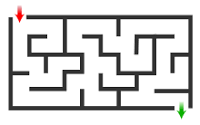
\includegraphics[width=6cm]{pic/maze.png}
\caption{Maze}
\label{Maze}
\end{figure}

Computer scientists have long known parallel computing is the way to speed up solutions to such problems. But how to realize parallel computing needs the help of physicists. Indeed, a physicist would suggest the following experiment to attack the problem: run water into the entrance and observe what's coming out of the exit. If we see water out of the exit, we know the maze has at least one good path. Of course, this is not the ultimate answer. But at least it shows the power of using water for parallel exploration.

\subsection{A blackbox maze problem}

\subsection{Encryption is a maze game}
Cryptographers have also known that all computationally difficult problems are candidates of encryption algorithms. What if Alice at the entrance of a maze has a way to select the path when putting a drop of water into the maze?  An onlooker who observes how the water drop exits cannot determine which path it has taken without trying out each possible path. But what if Bob, who some agreed knowledge with Alice, can differentiate the path taken by the water drop? The maze is an encrypted communication channel between Alice and Bob.

\section{The quantum power}
Playing with water tricks is exactly the idea behind quantum computing and communication. The fundamental concepts of quantum physics are in the so-called particle-wave dual nature: 1. all matters are waves even the seemingly size-less electrons and protons; 2. all waves have their smallest drops, which cannot be divided further.

The first hint of quantum power for parallel computing came by the proposal of Deutsch's algorithm\cite{1985Deutsch} although the shock did not come until the publication of Shor's algorithm in 1997. The hint of quantum application to secure communication came a year early in 1984 though by the publication of the BB84 protocol\cite{BB84}.

\subsection{What is a particle}
To most people, particles have the image of point like or of negligible sizes. This image excludes the wave nature from the picture and cause all the misunderstandings when learning quantum physics. It really refers to the fact that all matters have the smallest drops when measured certain ways. For electrons and protons, measurement of their mass or charge show the smallest drops. For photons, measure their energy show the smallest drops. Through out this book, we avoid using the mis-leading term particle and use "quantum" to refer to the smallest drop photons, electrons and protons.

\subsection{What is a wave?}


\subsubsection{Types of waves}

For communication, beside radio waves, we also use laser lights launched into optical waveguides such as optical fibers. They are confined in two dimensions -- the lateral dimensions -- but propagate in the dimension along the axis-es of the waveguides or fibers. Using waveguides, optical fibers in particular, allows us to guide the lights to other optical devices. For this type of waves, amplitude, frequency, phase and polarization are also their characteristics.

If a wave is confined in three dimensions, e.g. an electromagnetic wave in a microwave oven, the wave cannot propagate anywhere other than being reflected back. Only standing waves of specific frequencies can exist in the confinement. The allowed frequencies are discrete. Standing waves are good for storing information. Superconductor qubits are built by standing waves of electrons as we will describe further below. Standing waves may be best visualized and understood by the vibrations of a guitar string. When we pluck a string, the propagation of the vibrations are stopped and reflected by the two fixed ends. Only the waves whose phases coincide after a complete round trip of reflection survive while the other waves cancel each other and die off.

Another type of waves, which we may call trapped waves, are not confined but are trapped by forces extending to infinity. Electrons are trapped waves by the electric force of a nucleus' positive charges. The waves extend to infinity but are concentrated within a nanometer around the nucleus. Trapped waves are also good for storing information. Trapped-ion qubits are built by trapped electron waves.


\subsubsection{Controlling a wave}

To attack the final question of how many good paths there are, we would propose refining the experiment this way: run several water drops into the entrance and see how many drops will come out. Here, we run into the challenge of how to achieve the precision we need: if one drop comes out of the exit, how do we know whether there is only one good path or there are two drops from two paths arriving the exit at the same time. It would be ideal if we know what the smallest drop of water is like so that we can distinguish one drop from a big combined drop.

%\tdplotsetmaincoords{60}{120} % Set the viewpoint angles (adjust as needed)

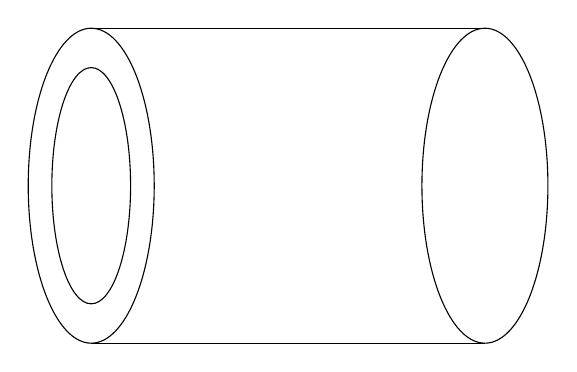
\begin{tikzpicture}%[tdplot_main_coords]
% Draw the outer surface of the tube
\draw (0,0) ellipse (0.8cm and 2cm);
\draw (5,0) ellipse (0.8cm and 2cm);

% Draw the inner surface of the tube (representing the hollow part)
\draw (0,0) ellipse (0.5cm and 1.5cm);

% Connect the ends of the cylinders to form the tube
\draw (0,-2) -- (5,-2);
\draw (0,2) -- (5,2);
\end{tikzpicture}


\subsubsection{Optical waveguide quantum computing chip}
If we take a look at the Xanadu.ai M-8 quantum computing chip, we see it very much ressembles a maze. The optical waveguides are the paths that light waves traverse. Its couplers and splitters ressemble the junctions of maze. A coupler merge two light paths into one, and a splitter split one into two. The chip has 8 entrances and 8 exits and can build $8^8$ possible paths.

Quantum physics tells us that all matters are waves and in addition, they all have the smallest drops, which cannot be divided finer when measured in their energy or mass. A wave, like water, can spread in space and propagate in time through all possible paths and give us the power of parallel computing. The drop-like behavior gives us the needed precision. Physicists refer the drop-like behavior the particle nature of matters. But the term particle unavoidably suggests minuscule in size and clarity in trajectory, and leads to avoidable puzzles and paradoxes with waves' spread in space and propagation in time. We should imagine or interpret electrons and electromagnetic waves like water drops: they can spread in space and propagate in time, may be subjected to constraints such as reflective objects, but show the smallest drops when measured by energy or mass.

\section{Quantum circuits and programming}

When implementing the algorithms and protocols in software, we first draw out them as quantum circuit diagrams. Our software programs would call out qubits for input and output as well as the gates for processing according to the circuit diagrams. Qubit stands for quantum bit. For quantum computing, a qubit is the data memory device that typically stores a bit of information to be processed. The storage medium is a drop of wave, and the device includes hardware that contain the wave. For quantum communication, a qubit is the channel uses one drop of wave to carry one bit of information. It is no difference from a radio wave or optical wave communication channel except it uses one drop of wave at a time. Appendix \ref{A-qubit} explains the physics behind the construct and operation principles of several types of qubit devices. In Chapter \ref{C-qi} on quantum information, we will revise the notion that a qubit can stores or carries only one-bit of information. Before that, we will stay with the qubit definition implied by its name and repeated in literature.

Conventional computers have no resemblance to quantum computers. Even before the appearance of modern computer, the not widely known subject of optical computing has explored the parallel computing capability of optical waves with Fourier transformation. But its application is limited and has not become a subject of learning by many. On the other hand, quantum devices have much in common with radio and optical communication devices because they all work with waves. Radio-wave communication including mobile communication and Wi-Fi is the dominating way for everyone connecting to the wired world. Mobile devices already take advantage of waves' parallel exploration capability for transmitters and receivers to find each other. The backbone of the wired world, on the other hand, is all optical fibers. The knowledge of wave communication reaches more engineering students than quantum physics and is most relevant not only to quantum communication but also to quantum computing. This chapter reviews some of the relevant subjects of communication theories especially on modulation before delving into the following chapters on the specifics of quantum communication and computing.

At the top level, a communication system has an information sender, a channel and a receiver. The sender contains modulators that transfer information in the form of numbers to characteristics of waves and send the waves to the channel. The receiver has demodulators that translate wave characteristics back to information. In a quantum system, the modulators and demodulators are quantum gates. The information bits carried in a quantum channel are called qubits -- short for quantum bits.

An ideal channel maintains the form and shape of the waves so that no information is lost. The equivalent in a computing system is a memory device, which receives bits of information from a writer and conveys them to the reader. Channels and memory devices, which work with quantum waves, are all qubit devices and may often be loosely referred as qubits.

Quantum gates are modulators and demodulators, and are not the same as transistor gates in a conventional computer. They convert information from one form of wave to another. A circuit of quantum gates would turn a maze of data (information) to an obvious form for easy extraction and achieve the task of computation. Or a circuit can turn the data (information) to an obscure form and achieve the task of secure communication.

When we talk about quantum computers, we should understand that we don't have entire computers made of all quantum devices. They will only have some chips or co-processors be replaced by chips of integrated circuits of quantum devices. Even our conventional computers have graphic processor units (GPU) in addition to the central processing units (CPU) to help speed up the processing of video display data.

\section{The quantum concepts}
For engineers, only two concepts of quantum physics are needed: 1. all matters are waves even the seemingly size-less electrons and protons are; 2. all waves have their smallest drops, which cannot be divided further. Physicists refer the two concepts the particle and wave duality of matters. In this book, we call the smallest drop of wave a quantum instead of a particle. To most people, particles have the image of point like or of negligible sizes. This image completely removes the wave nature from the picture and cause all the misunderstandings when learning quantum physics. We still call a quantum of light a photon and a quantum of electron waves an electron. We just avoid using the term particle.

The first concept tells us that, not limited to radio and optical waves, electrons and protons can also be used to make qubits.

The second concept is simple and easy to understand. But it leads to profound differences between a quantum wave and a classical wave -- one that has theoretical limit of dividing into smaller drops. The most profound difference is that one quantum of a wave can only be measured once. After measurement, the quantum of wave is no longer the same as it once was. This is the so-called Bohr quantum collapse theory. Another difference is that possible value of the measurement, in many circumstances such as the amplitude, can take only discreet values instead of a continuous range of values in the case of a classical wave. This difference relates to the so-called von Neumann projection theory. We shall explain these theories further when we encounter the relevant topics.

\chapter{Using waves to represent information}

\section{Optical waveguide qubits}
Another type of qubits uses lights confined in optical waveguides or fibers. We use the optical wave in waveguide A to represent the binary number 0 and label it $|0>$. We use the one in waveguide B to represent 1 and label it $|1>$. The two waves have the same frequency and amplitude. They don't overlap and are of course orthogonal to each other. If we bring the two waveguides together to overlap (using an optical coupler), we get a superposition wave that is a sum of both waves. If the sum has $cos\theta$ amount in amplitude from $|0>$ wave contributes and $sin\theta_p$ amount in amplitude from the $|1>$ wave, we can use the value $\theta_p$ to characterize the superposition wave.

\begin{figure}[ht]
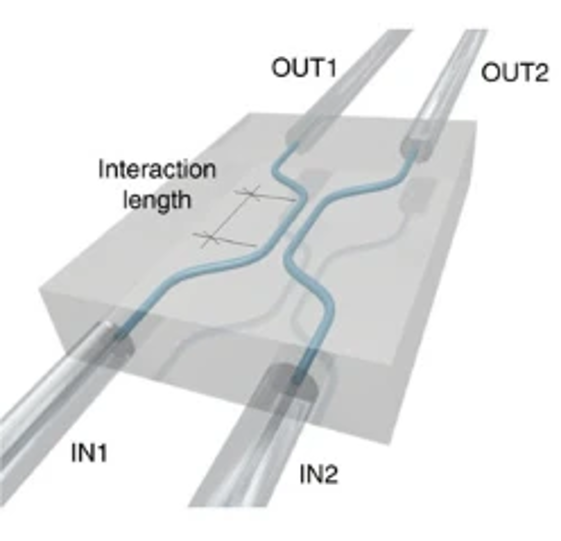
\includegraphics[width=6cm]{pic/wguideQubit.png}
\caption{Waveguide qubit}
\label{Waveguide}
\end{figure}

\section{Waves and modulation}
When talking about waves, we often visualize ripples in a lake or the surges in oceans and seas. We observe water being pushed up and then pulled down by gravity. When we shake one end of a string as show in Fig. \ref{String}, we also see the vibration of each section of the string and the propagation of the vibration. Our perception of a wave involves something vibrating and the vibration propagating. But can we consider the vibration of a guitar string as a wave? Indeed, we can. The reason we don't perceive the vibration propagating is because it gets reflected back by the two fixed ends of the string. Therefore, propagation or spatial spread remains a defining characteristic of waves, even if their propagation or spread is constrained.

Fig. \ref{String} shows, in the spatial dimensions $x$ and $y$, the speed $v$, wavelength $\lambda$ and the amplitude $y_0$ being the characteristics of the wave of the string. Shown but not labeled in the figure is the polarization of the vibration is in the $y$ direction. Vibration is a periodic motion, and in the time dimension, can be characterized by frequency and phase. Fig. \ref{wave} shows the period (the inverse of the frequency), phase and amplitude of a sinusoidal vibration when depicted in the time dimension. All these characteristics wavelength, amplitude, frequency, period and polarization can be modulated to represent information. But wavelength, frequency and period are related, and only frequency is used for modulation.

In radio wave communication, which includes mobile or cellphone communication we use everyday, the modulation of frequency, phase, and amplitude serves as the primary methods for information representation. In optical communication, combination of polarization and phase modulation is mostly used. In subsequent sections, we will find that quantum devices use all of them and others for information modulation.

\begin{figure}[ht]
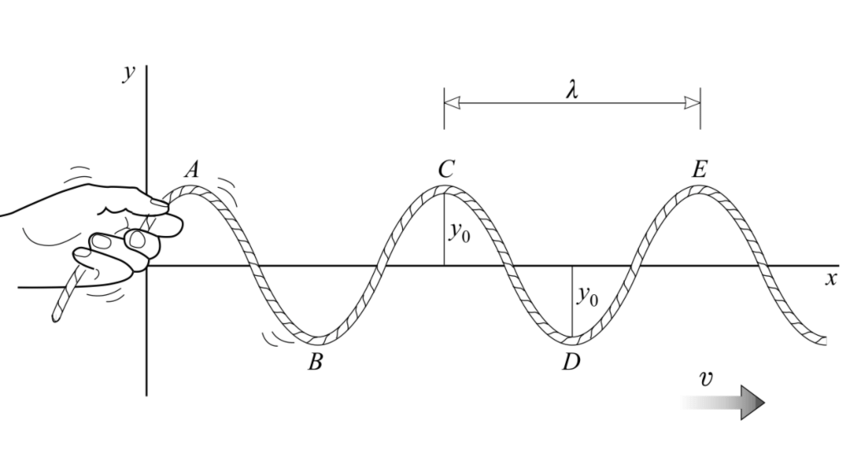
\includegraphics[width=6cm]{pic/wave-in-a-string.png}
\caption{Wave arisen from shaking or vibrating one end of a string.}
\label{String}
\end{figure}

\begin{figure}[ht]
\begin{tikzpicture}
    \draw[->] (-3.5,0) -- (3.5, 0);
    \draw[->] (0,-3.5) -- (0,3.5);
    \draw[dotted, red] (-3.5,0) sin (-2.5,3) cos (-1.5,0) sin (-0.5,-3) cos (0.5,0) sin (1.5,3) cos (2.5,0) sin (3.5,-3);
    \draw[red, fill] (-2.5,3) circle(0.05cm);
    \draw[red, fill] (1.5,3) circle(0.05cm);
    \draw[dashed] (-2.5,0) -- (-2.5,3) node[pos=0.5, rotate = 90, above] {amplitude};
    \draw[dashed] (-2.5,3) -- (1.5,3) node[pos=0.3, above] {period};
    \draw[red, fill] (0.5,0) circle(0.05cm);
    \draw[dashed] (0.25,-0.1) -- (1,-2) node[below] {phase};
\end{tikzpicture}
\caption{Characteristics of wave vibration}
\label{wave}
\end{figure}

\section{Information, numbers and modulation}
When we get our blood pressure measured in a doctor's office, the height of the mercury in a glass column represents 
the information of our blood pressure. The height of mercury in the column is what we actually measure and is 
what we use to represent the information of our blood pressure. We see that physical characteristics, which can be measured in numbers, can be used to represent information. Information theory assumes all information can be presented as numbers. In turn, engineers and physicists use physical characteristics that can be measured in numbers to represent the information. The whole process is
Information -> Numbers -> Wave characteristics. The first step is called encoding, and the second step is modulation.

In the study of communication, modulation is the subject devoted to how information or numbers being represented by physical characteristics of waves. The wealth of knowledge can be applied to not only quantum communication protocols but also to quantum computing.

Radio broadcasts first used radio waves' amplitudes to represent the volume of one's voice. This is the so called amplitude modulation (AM). Later, frequency modulation (FM) was found less prone to noise in the airways. That is why we now have both AM and FM on the panels of our radios. Modern communication also use phase modulation (PM) and quadrature amplitude modulation (QAM), which is a combination of phase and amplitude modulation.

Quantum devices, working with the smallest drops of waves, typically use two wave characteristics in their modulation scheme. Understanding how modulation works in quantum devices is the critical link for engineers to understand quantum technologies.

\subsection{Phase modulation}
Phase modulation uses a carrier wave's phase to represent information. By varying the phase while keep the wave's frequency and amplitude constant, the real numbers in the [0, 2$\pi$) domain can be represented. In communication textbooks, we use the points in constellation diagrams to depict the amplitudes and phases of waves -- 
the distance of a point to the origin is the amplitude of the wave, and the angle to the x-axis $\phi$ is the phase. 
So, the numbers that PM can represent fall all onto a circle in a constellation diagram as in Fig. \ref{PM}. Communication textbooks refer the numbers symbols. The range or set of the symbol is called the symbol constellation or symbol set. For example, the symbol constellation of PM in set notation is $phi in [0, 2\pi)$.
(Constellation diagrams are most useful for understanding QAMs, in which both amplitudes and phases are used to represent information.)

%\node [constellation_cir] at (0,0) {};
\begin{figure}[ht]
\begin{tikzpicture}
    \draw[->] (-3.5,0) -- (3.5, 0);
    \draw[->] (0,-3.5) -- (0,3.5);
    \draw[dotted, red] (0,0) circle(3cm);
    \draw[red, fill] (30:3) circle(0.05cm);
    \draw[dashed] (1,0) arc (0:30:1) node[right, pos=0.6]{$\varphi$ - phase};
    \draw[dashed] (30:0.1) -- (30:2.9) node[pos=0.5, rotate = 30, above] {amplitude};
\end{tikzpicture}
\caption{Constellation diagram of phase modulation}
\label{PM}
\end{figure}

\subsection{Digital modulation}
In theory, we can measure a wave's amplitude, frequency and phase precisely and use them to represent real numbers. In really, communication channels and information processing devices have noises and errors. We are best to have the systems working with only integer numbers. Using integer numbers to represent information is what we call digital technology. Further, using binary integers instead of decimals makes computer and communication components much simpler. And nowadays digital technology is almost the synonym of binary technology. Technologies of dealing with real numbers are called analog technologies.

All computers use digital technology if we ignore the history of the slide rule calculators. Even abacuses are digital calculators. Communication systems are slow to convert to digital technology. For a long time, communication was mostly about voice communication -- radio broadcast and telephones -- and used analog technologies. For digital information, modulations such as AM, FM and PM often carry different names, e.g. amplitude-shift keying (ASK), frequency-shift keying (FSK) and phase-shift keying respectively (PSK).

\subsection{Channel capacity and Hartley's law}
Channel capacity measures the maximum possible bits per second of a communication channel. When modulation is the only limitation, Hartley's law gives the channel capacity to be
\begin{equation}
    C = f ln M
\end{equation}
where $f$ being the channel used rate and $M$ being the number of modulation points.

\section{Quadrature phase-shift keying}
Quadrature phase-shift keying (QPSK) uses carrier waves of phases 90 degree apart, for example of phases 0, 90, 180, 270 degrees, to represent 2-bit numbers -- 0, 1, 10, or 11 in binary. A wave with 90 degree phase is called the quadrature wave while the wave with zero phase is called the in-phase wave.
(The significance of using waves with phases 90 degree apart is that every two waves of such phase difference are orthogonal to each other. Therefore, when receiving a wave of phase 180 degree representing "10", which has zero measurement overlap with waves of 90 or 270 degree phases, and has zero probability of being demodulated as "1" or "11".
waves are orthogonal to each other. Measurement of orthogonal waves is least prone to noise or errors 
because they have zero overlap.)

The constellation diagram is shown in the left diagram in \ref{4QPSK}.

\begin{figure}[ht]
\begin{tikzpicture}
    \draw[->] (-3.5,0) -- (3.5, 0);
    \draw[->] (0,-3.5) -- (0,3.5);
    \draw[dotted, red] (0,0) circle(3cm);
    \draw[red, fill] (3,0) circle(0.05cm) node[below right] {0};
    \draw[red, fill] (0,3) circle(0.05cm) node[above right] {1};
    \draw[red, fill] (-3,0) circle(0.05cm) node[above left] {10};
    \draw[red, fill] (0,-3) circle(0.05cm) node[below left] {11};
\end{tikzpicture}
%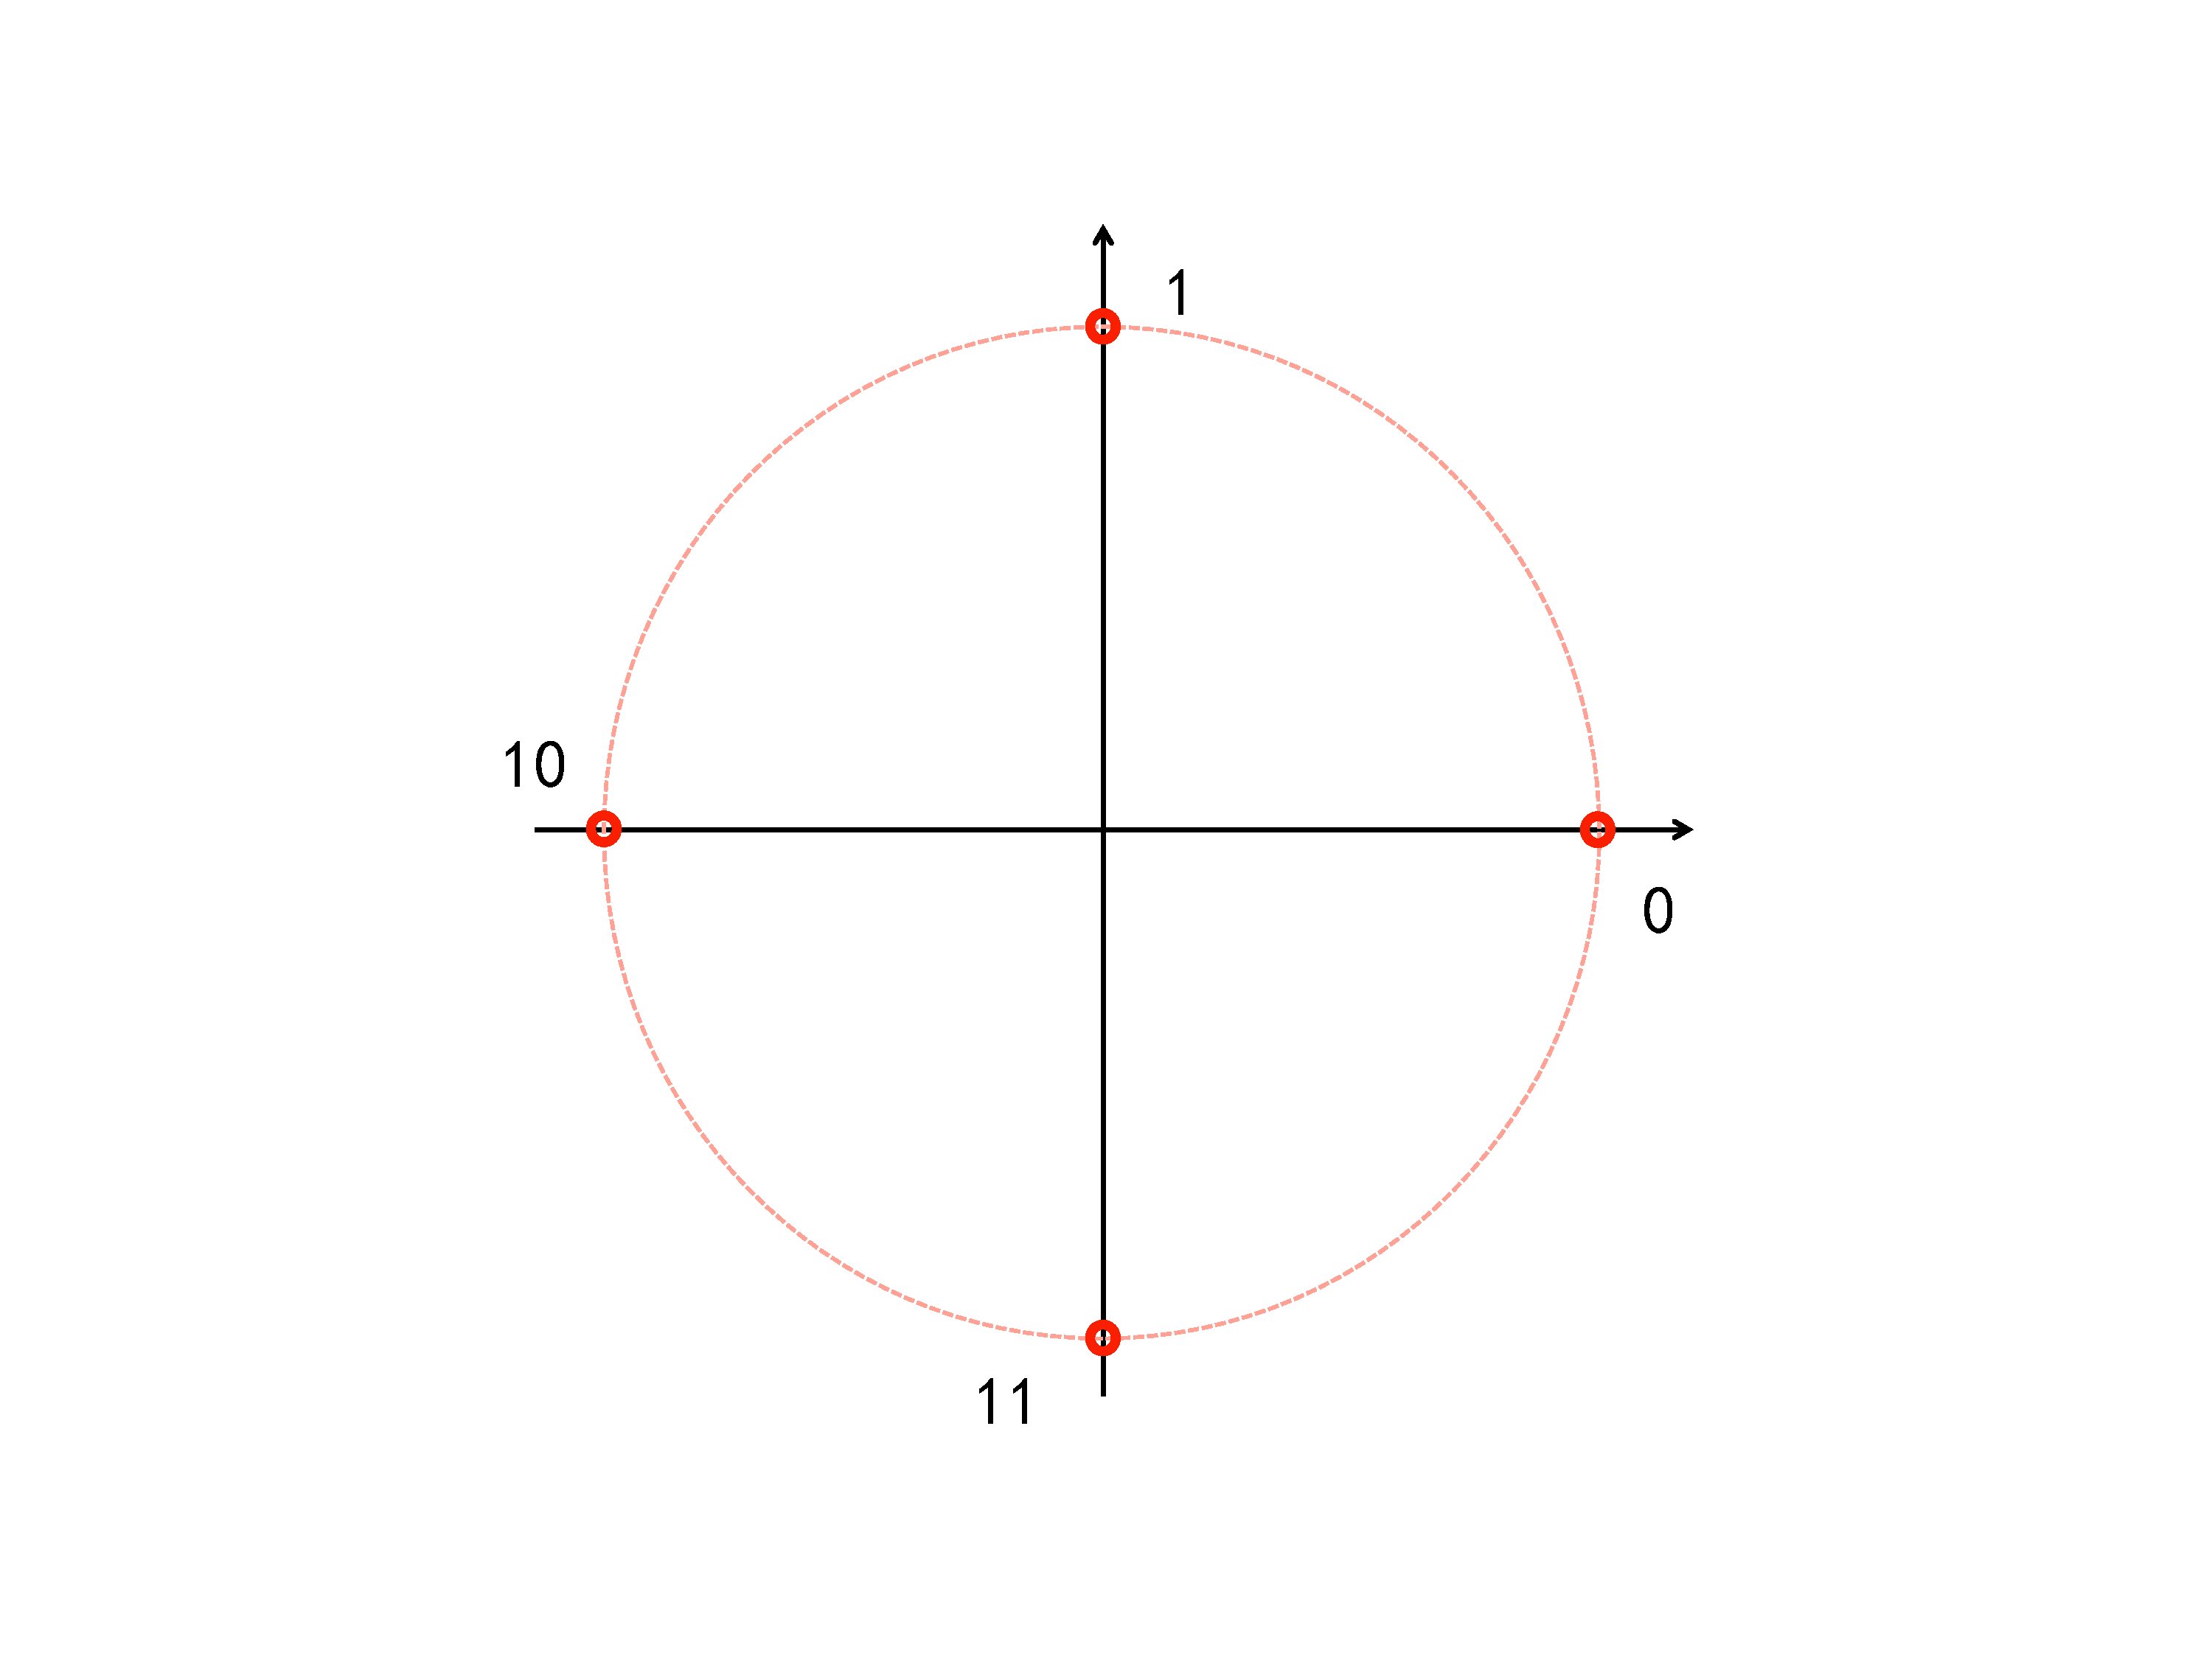
\includegraphics[width=6cm]{pic/4qpsk.pdf}
\caption{QPSK constellation diagram}
\label{4QPSK}
\end{figure}

\subsection{Symmetric QPSK}
For simpler modulator circuitry, the QPSK modulation scheme shown in the constellation diagram Fig. \ref{QPSK} is more widely used in practice.
\begin{figure}[ht]
\begin{tikzpicture}
    \draw[->] (-3.5,0) -- (3.5, 0);
    \draw[->] (0,-3.5) -- (0,3.5);
    \draw[dashed] (2.5,2.5) -- (-2.5,-2.5);
    \draw[dashed] (-2.5,2.5) -- (2.5,-2.5);
    \draw[dotted, red] (0,0) circle(3cm);
    \draw[red, fill] (2.12,2.12) circle(0.05cm) node[right=5] {11};
    \draw[red, fill] (-2.12,2.12) circle(0.05cm) node[above=5] {01};
    \draw[red, fill] (2.12,-2.12) circle(0.05cm) node[below=5] {00};
    \draw[red, fill] (-2.12,-2.12) circle(0.05cm) node[left=5] {10};
    \draw[dashed] (1,0) arc (0:45:1) node[right, pos=0.6]{$\varphi=\pi/4$};
\end{tikzpicture}
%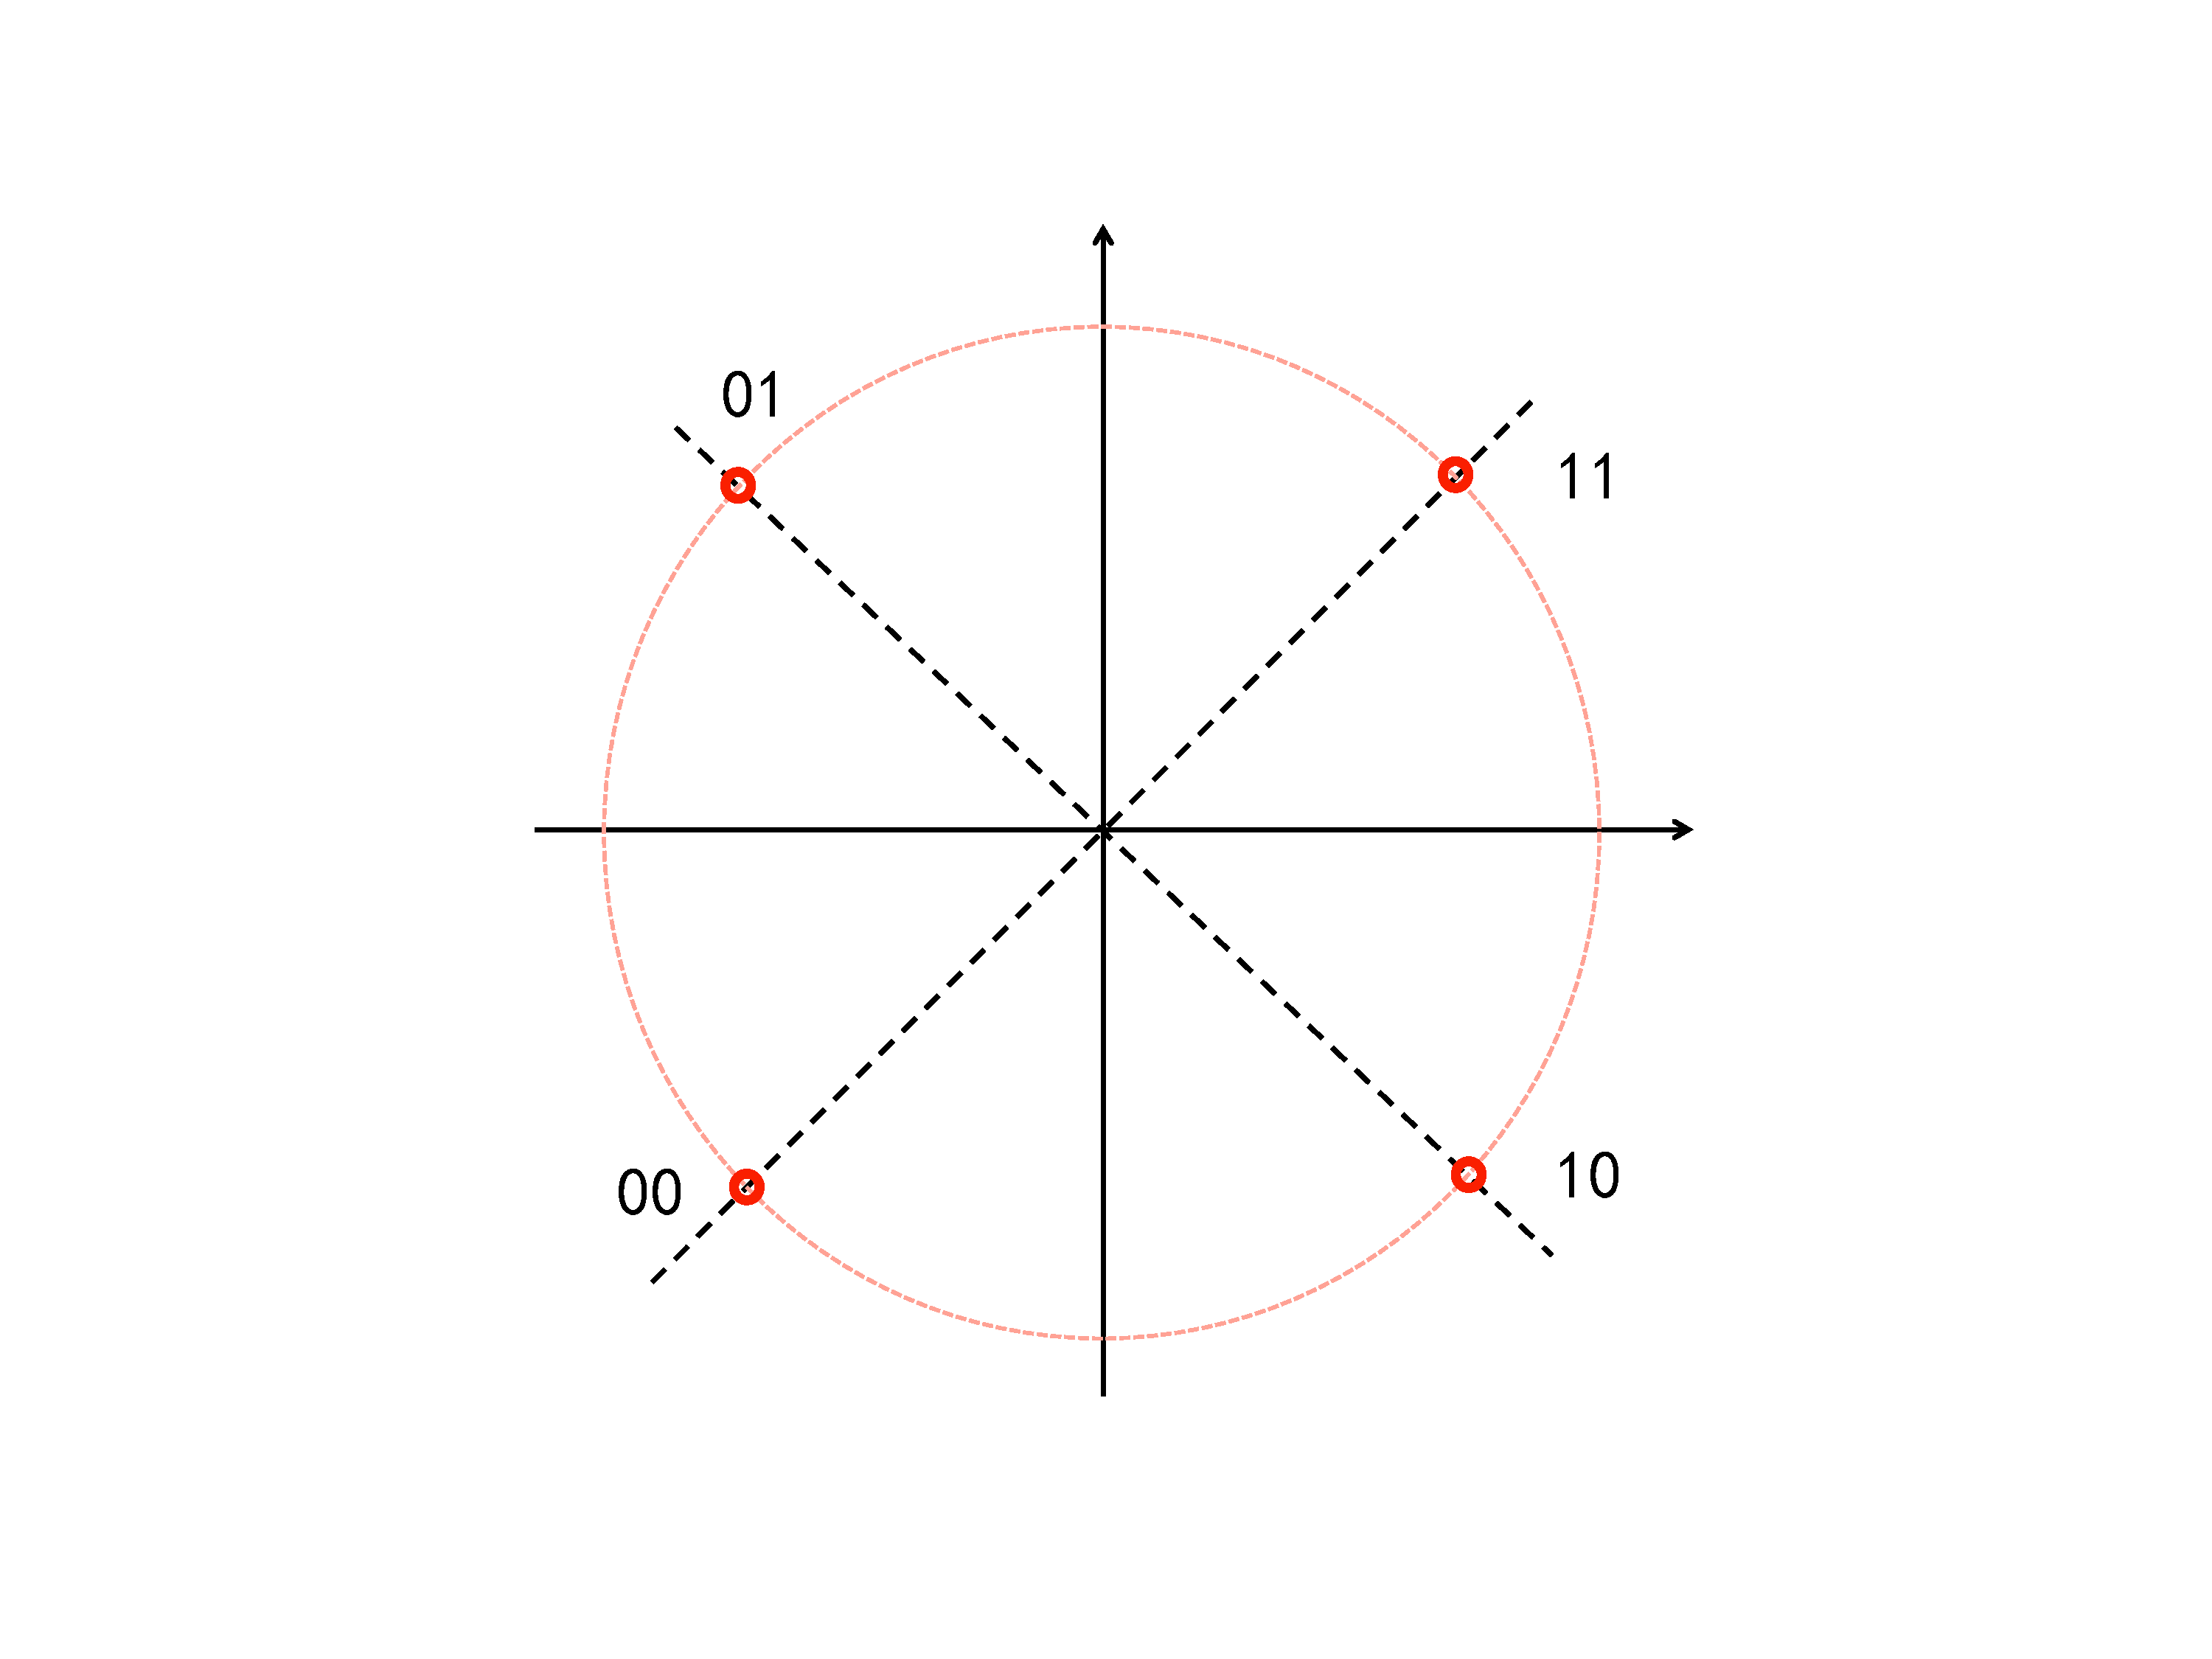
\includegraphics[width=6cm]{pic/qpsk.pdf}
\caption{Practical QPSK constellation diagram}
\label{QPSK}
\end{figure}

\subsection{Modulator, demodulator and superposition}
A practical QPSK modulator circuit is shown in Fig. \ref{modulator}. It uses one carrier wave generator and splits the carrier wave into two waves of equal amplitudes. One of the half becomes the quadrature wave after a 90-degree phase shifter while the other half remains as the in-phase wave. modified scheme: in every time slot, 2 bits are fed into the modulator. Each bit is used to modulate a base carrier wave's phase. The two base carrier waves are orthogonal, one of zero phase and the other of 90-degree in phase. If the input to a carrier is "0", its phase is shifted another 180 degrees. The combined or summed up wave of the two carriers is the output of the modulator going into the communication channel. The constellation diagram this scheme is shown in Fig. \ref{QPSK}.

We see that one wave from the source can be divided up into two waves, which can then be combined into one after modulation. In fact, all waves can be combined into one and may be regarded as one wave if they are coherent with each other -- their phases are correlated. Combination, mixing or composing several waves into one is the same concept as superposition in quantum physics although the latter refers to combination, mixing or composition of waves with equal number of drops.

\begin{figure}[ht]
\begin{tikzpicture}
    \path %(-5,0) node[anchor=east] (start) {Wave} 
    (-3.5,-0.8) node[circle, draw=black] (lo) {$\sim$}
    (-3.5,0.8) node[Gate] (p90) {$90^\circ$}
    (0,2) node[Gate, text width=30] (tm) {$0/180^\circ$}
    (0,-2) node[Gate, text width=30] (bm) {$0/180^\circ$}
    (2,0) node[circle, draw=black] (add) {+}
     (3,0) node[anchor=west] (output) {wave output};
    \draw (lo.east) node[anchor=west] {carrier wave generator};
    \draw (p90.east) node[anchor=west] {phase shifter};
    \draw (tm.north east) node[anchor=west] {variable phase shifter};
    \draw (bm.south east) node[anchor=west] {variable phase shifter};
    \draw (lo) -- (p90) |- (tm) -| (add);
    \draw (lo) |- (bm) -| (add);
    \draw (add) -- (output);
    \path (-2,3) node[anchor=east] (even) {data input - even bits}
    (-2,-3) node [anchor=east] (odd) {data input - odd bits};
    \draw[double] (even) -| (tm);
    \draw[double] (odd) -| (bm);
\end{tikzpicture}
\caption{QPSK modulator circuit}
\label{modulator}
\end{figure}

Figure \ref{deodulator} shows a demomulator circuit, which reverses the modulation: the received signal wave is divided into two waves to be resonated with two local oscillators, which are from the same local source but are orthogonal to each other. The the proportions of the two resonations determine the phase angle of the incoming wave. Bit numbers are output according to the phase angle.

\begin{figure}[ht]
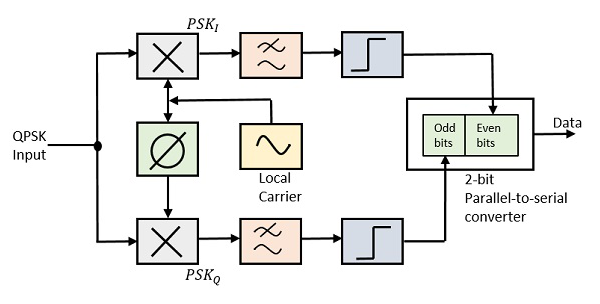
\includegraphics[width=6cm]{pic/qpsk_demodulator.jpg}
\caption{QPSK demodulator circuit}
\label{deodulator}
\end{figure}

\section{Quadrature amplitude modulation}
Quadrature amplitude modulation (QAM) is a combination of amplitude modulation and phase modulation. Modern radio communication such as Wi-Fi and mobile communications all use the digital forms of QAMs.
\begin{figure}[ht]
\begin{tikzpicture}
    \draw[->] (-3.5,0) -- (3.5, 0);
    \draw[->] (0,-3.5) -- (0,3.5);
    \draw[dotted, red] (0,0) circle(3cm);
    \draw[red, fill] (2,0) circle(0.05cm) node[below] {0};
    \draw[red, fill] (0,2) circle(0.05cm) node[right] {1};
    \draw[red, fill] (-2,0) circle(0.05cm) node[above] {10};
    \draw[red, fill] (0,-2) circle(0.05cm) node[left] {11};
    \draw[red, fill] (3,0) circle(0.05cm) node[below right] {100};
    \draw[red, fill] (0,3) circle(0.05cm) node[above right] {101};
    \draw[red, fill] (-3,0) circle(0.05cm) node[above left] {110};
    \draw[red, fill] (0,-3) circle(0.05cm) node[below left] {111};
\end{tikzpicture}
\begin{tikzpicture}
    \draw[->] (-3.5,0) -- (3.5, 0);
    \draw[->] (0,-3.5) -- (0,3.5);
    \draw[dashed] (2.5,2.5) -- (-2.5,-2.5);
    \draw[dashed] (-2.5,2.5) -- (2.5,-2.5);
    \draw[dotted, red] (0,0) circle(3cm);
    \draw[red, fill] (45:2) circle(0.05cm) node[above left] {11};
    \draw[red, fill] (135:2) circle(0.05cm) node[above right] {01};
    \draw[red, fill] (225:2) circle(0.05cm) node[above left] {00};
    \draw[red, fill] (-45:2) circle(0.05cm) node[above right] {10};
    \draw[red, fill] (45:3) circle(0.05cm) node[right] {111};
    \draw[red, fill] (135:3) circle(0.05cm) node[left] {101};
    \draw[red, fill] (225:3) circle(0.05cm) node[left] {100};
    \draw[red, fill] (-45:3) circle(0.05cm) node[right] {110};
\end{tikzpicture}
\caption{Constellation diagrams of two 8QAM systems}
\label{8QPSK}
\end{figure}

\section{Polarization modulation}
Polarization modulation is used in optical fiber communication. For example, dual polarization quadrature phase shift keying (DP-QPSK) modulation is a widely used.

\chapter{Quantum information}\label{C-qi}
\section{Quantum concepts}
For engineers, only two concepts of quantum physics are needed: 1. all matters are waves even the seemingly size-less electrons and protons are; 2. all waves have their smallest drops, which cannot be divided. Physicists refer the two concepts the partical and wave duality of matters. The first concept tells us that, not limited to radio and optical waves, electrons and protons can also be used to make qubits. However, the implication of the second concept is far more profound and is not explored by traditional communication theory:

\begin{itemize}
    \item Analog AM is not possible because amplitude depends on the number of drops in the wave and can only be use for digital modulation. 
    \item Each qubit can only be measured once. In disregard how many bits of information are modulated into a qubit, only one bit at most can be demodulated from a qubit.
\end{itemize}

\subsection{Measurement and limit on channel capacity}
When measuring a wave's mass or energy, we find it in a discrete number -- 1, 2, ..., or $n$ -- of a unit mass or energy. The one with 1 unit is the smallest drop of course. The amplitude is usually proportional to the square root of the mass or energy and takes only discrete values although not exactly 1, 2, ... or $n$.

When we have a wave of $n$ drops, we can divide it up to $n$ drops for separate measurements. But with measurement of each drop, the drop of the wave is changed or even disappears. A drop of an electromagnetic wave is called a photon. When measuring a photon, its energy is transferred to an electron, and the movement or change in the electron of charge induce an electrical current observable to humans. The photon cannot be divided and disappears after its whole energy is transferred to an electron. The unique feature of quantum information is that we can modulate a qubit device as much information as the cardinal of real numbers but that we can only extract at most one bit of information when measuring it.

\subsection{Quantum terminology}
By tradition, physicists keep on using the term particle, which may cause the biggest confusion. To most people, particles have the image of point like or of negligible sizes. Physicists believed electrons were point-like in size when JJ Thomson discovered them in 1897. But when Ernest Rutherford discovered atomic nucleus 14 years later, people raised the question: why is the size of an atom much bigger than that of its nucleus? Why wouldn't the tiny negatively charged electrons fall into the positively charged nucleus and be combined into an atom close to the size of the nucleus -- if it were to happen, we would have not seen the world as we have.

Physicists refer the drop-like behavior of electrons and all other matters as the particle behavior. "Quantum" should have been the perfect word in place of particle, but we think "drop" is a better word for non-physicists to understand.

Beside particle, physicists use the term "state" to refer the wave of one drop. It is the same concept as "mode" in the context of optical communication and photonics. It is used to describe a wave when the absolute amplitude value is known or unimportant. But the term carries many different meanings to engineers. We will believe it's wise to use the term "wave" in place of state. By tradition, physicists use the so-called Dirac "bra-ket" notation to label quantum states. In the ket notation, the base carrier waves are noted as $|0>$ and $|1>$.

When talking about electrons being waves, people are often puzzled and ask what is vibrating in an electron wave. Physicists are puzzled too and have been debating the possibilities without conclusion. Engineers don't have to interject into the debate and need only know that an electron wave qubit has frequency, phase and polarization for modulating.

\section{Qubit modulation}
\subsection{Requirements on modulation}
We have two conflicting requirements when considering how to modulate a qubit:
\begin{itemize}
    \item For parallel computing/exploration, the modulation code space should be as large as possible.
    \item For output, demodulated codes are limited to binary "0" and "1".
\end{itemize}

The first requirement is easy to understand, and analog PM, with symbol set $\phi in [0, 2\pi)$, meets the requirement. The second requirement is due to that fact that one qubit has only one drop wave, which resonates with only one of the local oscillators in the demodulator as shown in Fig. \ref{deodulator} and never both.

As described in the Appendix on qubit devices, all devices add polarization modulation or the like to meet the second requirement. (That's because polarization demodulation is easier than phase demodulation.) Polarization modulation is widely used in optical fiber communication. But some qubit modulation schemes such as using waveguide location have never been used in communication. And communication theory has no established terms for them. In this book, we refer them with a generic term $\theta$ modulation because all of them can be characterized by an angle value $\theta in (-\pi/2, \pi/2]$ as discussed in the appendix on qubit devices.

\subsection{Digital modulation}
\subsubsection{For output}
To read out from a qubit, it must be in a binary modulation. Similar to QPSK shown in Fig. \ref{4QPSK}, we use the angles $\theta=0$ and $\pi/2$ to represent "0" and "1" respectively as shown in the constellation diagram Fig. \ref{qQPSK} 
\begin{figure}[htbp]
\begin{tikzpicture}
    \draw[->] (-3.5,0) -- (3.5, 0);
    \draw[->] (0,-3.5) -- (0,3.5);
    \draw[dashed] (2.5,2.5) -- (0,0);
    \draw[dashed] (0,0) -- (2.5,-2.5);
    \draw[dotted, red] (0,0) circle(3cm);
    \draw[red, fill] (3,0) circle(0.05cm) node[below right] {0};
    \draw[red, fill] (0,3) circle(0.05cm) node[above right] {1};
    \draw[red, fill] (2.12,2.12) circle(0.05cm) node[right=5] {11};
    \draw[red, fill] (2.12,-2.12) circle(0.05cm) node[below=5] {10};
    \draw[dashed] (1,0) arc (0:45:1) node[right, pos=0.6]{$\theta=\pi/4$};
\end{tikzpicture}
%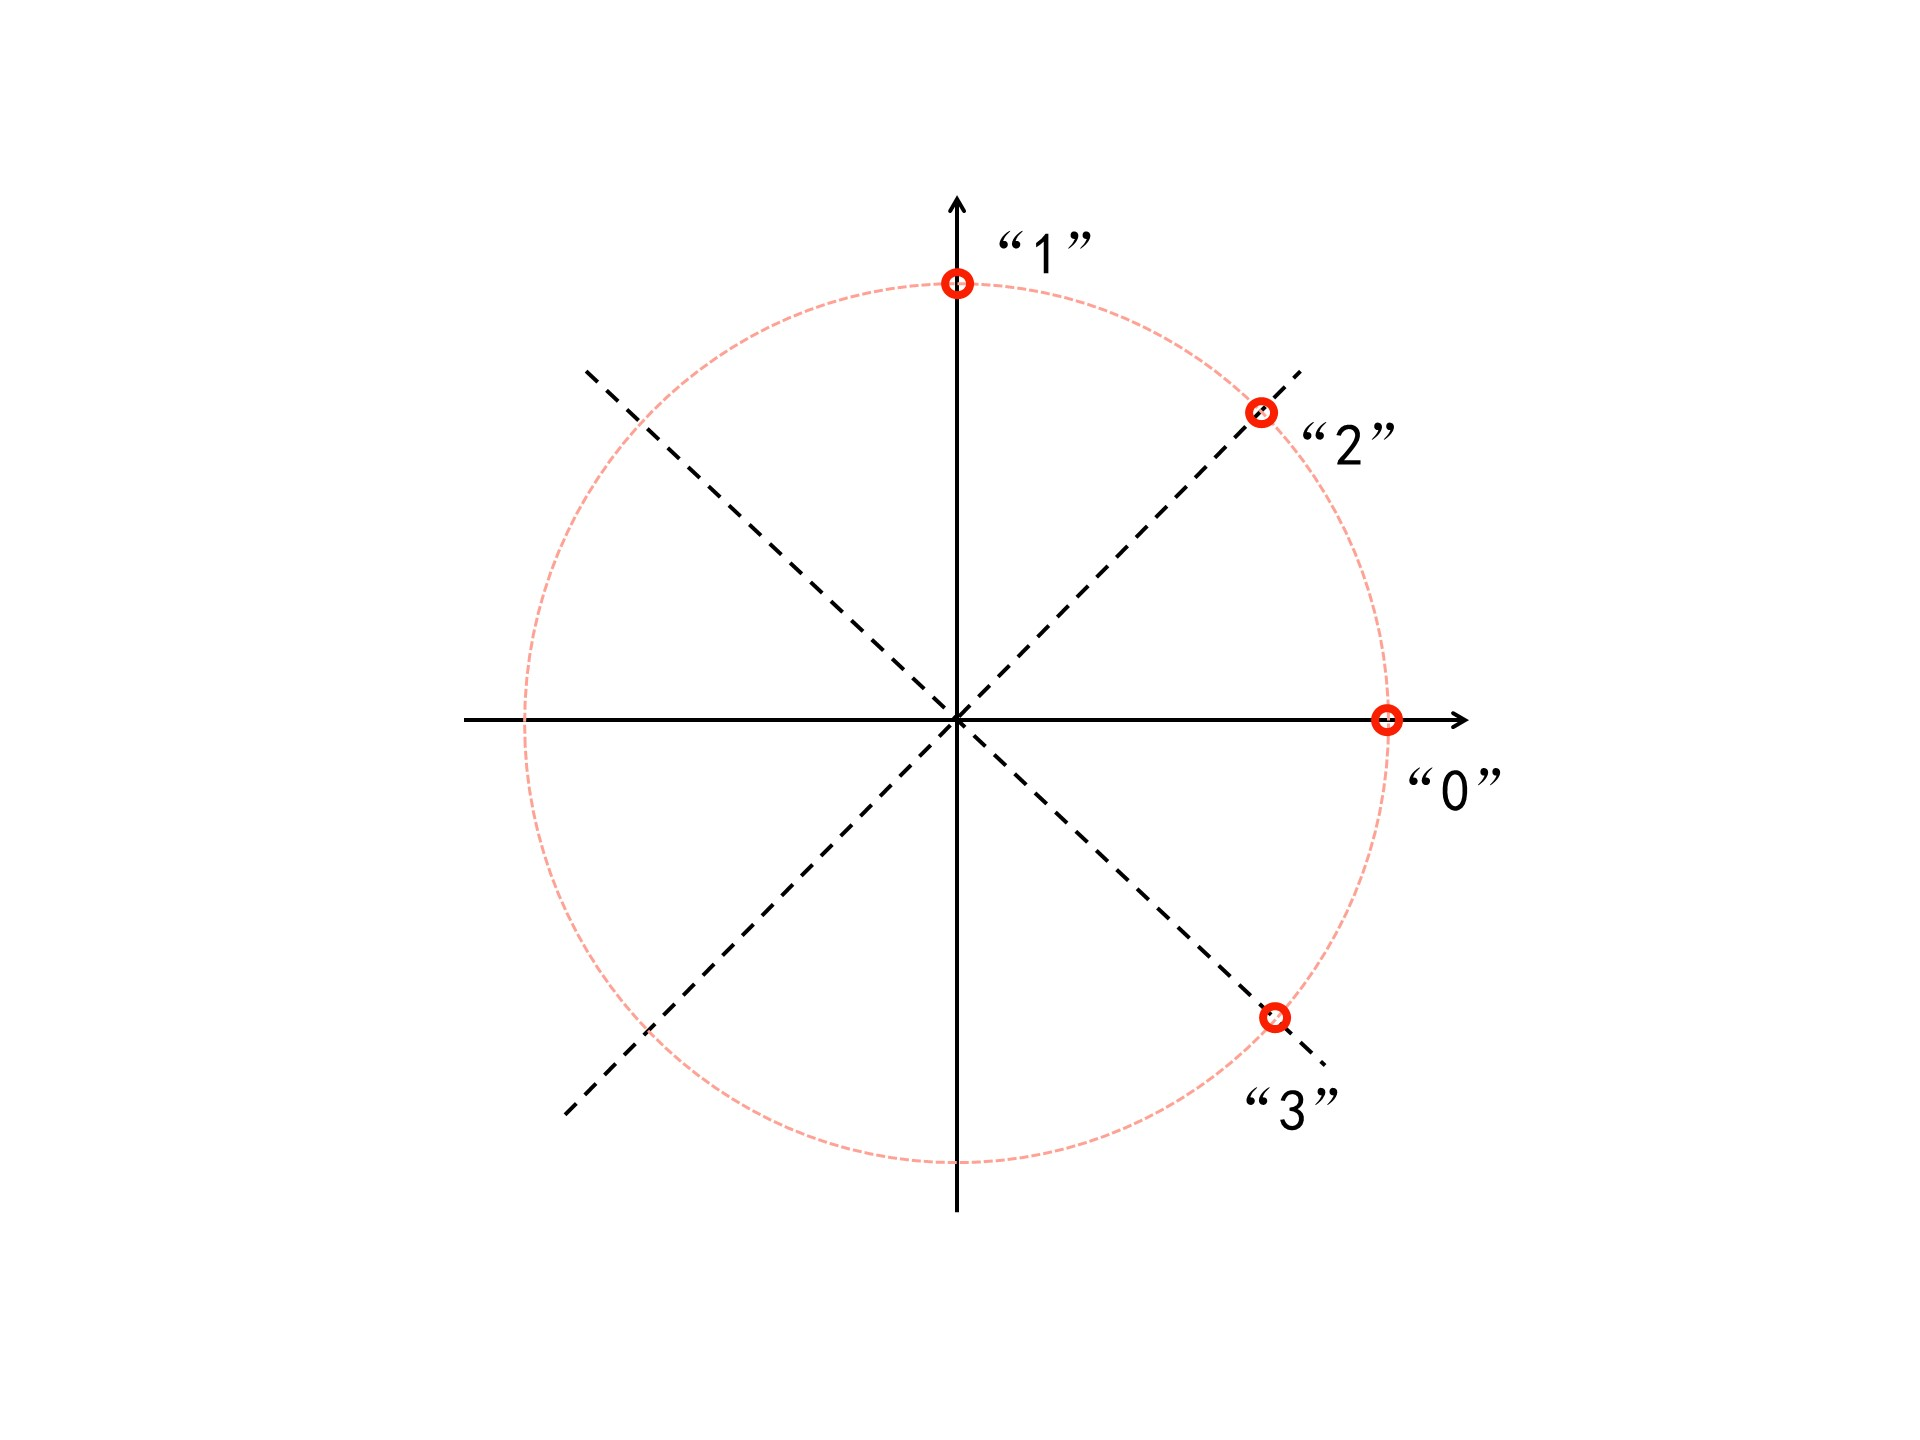
\includegraphics[width=6cm]{pic/qqpsk.jpg}
\caption{Constenlation diagram of quantum $\theta$ shift keying}
\label{qQPSK}
\end{figure}

\subsubsection{For input}
At the input stage of a circuit, we can also use the $\theta=\pi/4 and -\pi/4$ code points. They are called the Bell states by physicists. As we will learn in latter chapters, these waves can be used for parallel computing because each of them is a mixture or superposition of both he "0"ed "1" waves. For quantum communication, they encode the binary numbers "11" and "10", and are used as encrypted code points of one-time pad encryption.

\subsubsection{Quadrature amplitude modulation}
Since a wave is in drops, 1, 2, 3, ..., or n drops, its amplitude is discrete too although not in increment of 1, 2, 3, ..., or n. Adding amplitude modulation is by adding more qubits and can be used only for digital modulation. Amplitude modulation is always used to add code points for digital modulation and cannot be used for parallel computing.

\begin{figure}[ht]
\begin{tikzpicture}
    \draw[->] (-3.5,0) -- (3.5, 0);
    \draw[->] (0,-3.5) -- (0,3.5);
    \draw[dotted, red] (0,0) circle(3cm);
    \draw[red, fill] (2,0) circle(0.05cm) node[below right] {0, first qubit};
    \draw[red, fill] (0,2) circle(0.05cm) node[above right] {1};
    \draw[red, fill] (3,0) circle(0.05cm) node[below right] {10, second qubit};
    \draw[red, fill] (0,3) circle(0.05cm) node[above right] {11};
\end{tikzpicture}
\caption{Constellation diagrams of two qubits}
\label{QAM}
\end{figure}

(Ignore - If we consider the relative amplitude $A$ and phase $\phi$ of the two waves in a qubit, they can represent all the real number pairs in the rectangle ${ A \in [0,1], phi \in [0,2\pi) }$. Physicists like to represent the relative amplitude as $cos\theta$, and therefore, the $(\theta, \phi)$ pair can represent all the real number pairs in the rectangle ${[0,\pi],  [0,2\pi)}$. This rectangle can also be represented as a Bloch sphere.

\subsection{Analog modulation}
Analog modulation can only be used at input or in processing. For communication, each qubit actually has two channels -- $\theta$ and $\varphi$. And their channel capacities per qubit duty cycle are $\theta in (-\pi/2, \pi/2] and \varphi in [0, \pi)$. For computing, that is the capacities are the amount of information a qubit can store.

\subsection{Demodulation and quantum measurement}
When a cellphone receives a radio wave, the demodulator can divide the wave into many portions to measure the amplitudes and phases. But with a qubit, although we can adopt any of the modulation technique and put information in any of the data points $(\theta, \varphi)$, we cannot divide one drop of wave for multiple measurement.

Similar to a demodulator of QPSK. a demodulator of a qubit expose the drop of wave to two electronic resonators orthogonal to each other.  If we know the qubit is modulated by BQSK, detecting the qubit in the $|0>$ wave means the qubit's phase $\theta = 0$. Further, the absence of detecting signal in the $|1>$ wave also suggests $\theta = 0$ too. But if the qubit is originally modulated in any other way, we have no way of measuring the knowing the information that the qubit represents. the probability of one resonator responds to the wave depends on how much the resontor overlaps with the wave in space and time.

In contrast to conventional communication and computing systems, information entered into a quibit may be lost at demodulation or measurement. That is the unique feature of quantum information.

\section{Mathematical notation of qubit modulation}
From communication theory perspective, a qubit is best described by the parameter pair $(\theta, \varphi)$. But other notations developed by physicists may be easier to use when working on problems involving more than one qubit. 
\subsection{Ket notation}
Summing up the base carriers, the superposition wave can be noted as $|s> = cos{\theta} |0> + e^{i \varphi} sin{\theta}$ or simply $ |1>$ $|s> = a |0> + b |1>$. Here, the $+$ sign means wave addition but has no mathematical meaning. And $a$ and $b$ are complex numbers and reflect the amplitude and phase contributions to the superposition. Even with the constraint $|a|^2+ |b|^2$, this notation includes waves $e^{i\lambda} (cos{\theta} |0> + e^{i \varphi} sin{\theta})$ which are the same except their global phase $\lambda$.

\subsection{Vector notation}
For mathematicians and computer scientists, the physical meaning of wave addition can be ignored, and the vector notation $
\begin{pmatrix}
    a \\
    b
\end{pmatrix}$ is best for derivation and calculation.

But not all of the 4 real numbers the two complex numbers can be used independently for modulation. First, the amplitude of the wave is one to be sure that the qubit contains only one drop $|a|^2 + |b|^2 = 1$.
\begin{equation}
    \begin{pmatrix}
    cos\theta & -e^{i\lambda} sin\theta \\
    e^{i\varphi} sin\theta & e^{i(\varphi + \lambda)} cos\theta
\end{pmatrix}
\end{equation}
Any operation rotates the data point of a qubit on the Bloch sphere and can be described by the triplet of Euler angles, $\delta \theta, \delta \varphi, \delta \lambda$. The matrix notation is
\begin{equation}
    \begin{pmatrix}
        cos\delta \theta & -e^{i\delta lambda} sin\delta \theta \\
        e^{i \delta \varphi} sin\delta \theta & e^{i \delta \varphi+ \delta \lambda} cos\theta 
    \end{pmatrix}
\end{equation}

\subsection{Binary numbers}

If we measure waves in any other way than space or time, we find their smallest "drops" -- the particle nature of matter. Quantum physics started a hundred years ago when Einstein first proposed that electromagnetic waves, when measured in their energy, have the smallest drops called photons.

When measuring in electric charge, physicists discovered the smallest drops first and call them electrons before they realized their wave nature.

Measurement is the very thing that the quantum world is different from the classical world. In the quantum world, with an article, you only have one chance to measure it.)

Digital technologies gain precision over analog technologies but lose in the amount of information they can carry. The amount of information that a modulation technique can carry relates to the size or cardinality of the set of numbers that it can represent. With analog PM, the cardinality of the set [0, 2$\pi$) is infinity and is the same as the entire set of real numbers. But the set of integers that a digital modulation represent is finite. And the amount of information that a digital communication channel carries per time slot is finite. To increase the communication speed, the cellphone industry has been trying to squeeze more and more information per time slot by adopting increased data points of QAM modulations -- 4QAM, 8QAM, 16QAM ....
From the above description of the various types of qubits, we see that they all have the pseudo phase $\theta_p$ to characterize the 
orthoganility or overlap among the waves in the polarization, spatial or frequency domains, and can be used represent real numbers in the $\{\theta_p \in [0, \pi/2)\}$ domain. In addition, the relative phase in the time domain of the two base carrier waves in a qubit is another independent variable that can be. Physicists usually use $\theta_q = \theta_p/2 |0>$ and the Bloch sphere as in Fig. \ref{Bloch} to draw an intuitive picture of the entire modulation domain of a qubit $\{\theta_q \in [0, \pi]$ and $\phi \in [0, 2\pi)\}$.

\begin{table}[]
\caption{Parameters and ranges for modulation}
\label{modulation-parameters}
\begin{tabular}{lll}
Parameter &Represented numbers &Note                 \\
Amplitude &Number of qubits $\in \{1, 2, 3, ...\}$   & None \\
Phase & $\varphi \in (-\pi /2, \pi /2] $& Z gate \\
Polarization angle (spatial overlap) & $\theta \in (-\pi /2, \pi /2]$ &X gate
\end{tabular}
\end{table}

\section{Graphical depictions}
\subsection{Quarter sphere diagram}
\begin{figure}[ht]
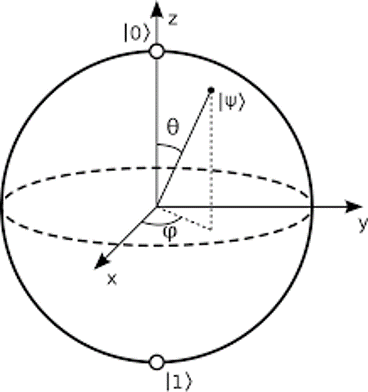
\includegraphics[width=6cm]{pic/blochSphere.png}
\caption{Bloch sphere}
\label{Bloch}
\end{figure}

\begin{figure}[ht]
\tdplotsetmaincoords{0}{0}
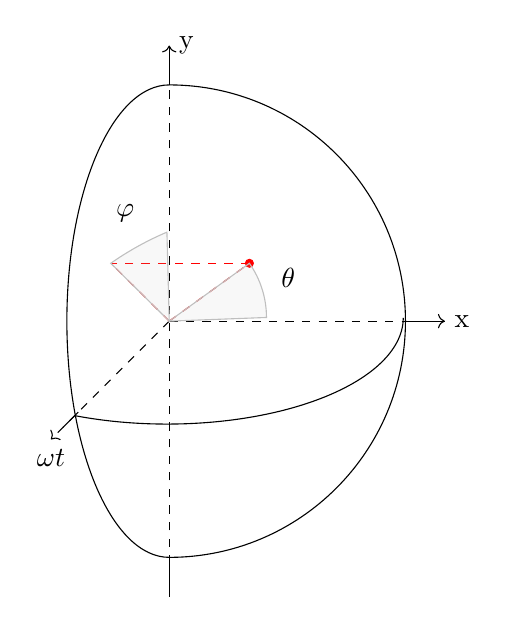
\begin{tikzpicture} %[scale=2,tdplot_main_coords]
 \def\rvec{3}
 \def\thetavec{50}
 \def\phivec{40}
 
    %Axes
    \coordinate (O) at (0,0,0);
    \draw[dashed, ->] (0,0,0) -- ++(3.5, 0,0) node[below,right] (x) {x};
    \draw[dashed, ->] (0,-3.5,0) -- ++(0, 7, 0) node[above,right] (y) {y};
    \draw[dashed, ->] (0,0,0) -- ++(0, 0, 3.9) node[below] (z) {$\omega t$};
    \draw[] (0,-3) arc(-90:90:3 and 3);
    \draw[] (0,3) arc (90:270:1.3 and 3);
    \draw[] (-1.2,-1.2) arc (-113:0:3 and 1.35);
    \draw[] (3,0,0) -- ++(0.5, 0, 0);
    \draw[] (0,-3.5,0) -- ++(0, 0.5, 0);
    \draw[] (0,3,0) -- ++(0, 0.5, 0);
    \draw[] (0,0,3) -- ++(0, 0, 0.5);

    % Vector
    \tdplotsetcoord{P}{\rvec}{\thetavec}{\phivec}
    \draw[red,fill] (P) circle(0.05);
    \draw[dashed, red] (O) -- (P) node[circle] (Ptheta) {};
    \draw[dashed, red] (O) -- (Pyz) node[circle] (Pphi) {};
    \draw[dashed, red] (P) -- (Pyz);
    %\draw[dashed, red] (Px) -- (Pxz);

    % angles;
    \draw [shift={(0,0)}, lightgray, fill, fill opacity=0.1] (0,0) -- (P) arc (35:0:1.2) -- cycle;
    \draw [shift={(0,0)}, lightgray, fill, fill opacity=0.1] (0,0) -- (Pyz) arc [start angle=125, delta angle=-12, radius=3.9 ] -- cycle;
    %\draw [shift={(0,0)}, lightgray, fill, fill opacity=0.1] (0,0) -- (Pyz) arc (75:60:1.2) -- cycle;
    \draw( -0.8, 1.6) node[anchor=north west] {$\varphi$};
    \draw( 1.3, 0.8) node[anchor=north west] {$\theta$};
\end{tikzpicture}
\caption{Qubit modulation space}
\label{bloch-alt}
\end{figure}

\subsection{Bloch sphere}
\begin{figure}[ht]
\tdplotsetmaincoords{0}{0}
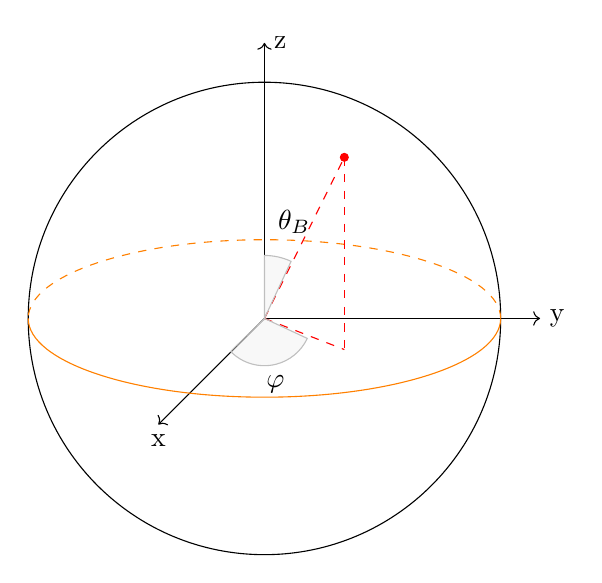
\begin{tikzpicture} %[scale=2,tdplot_main_coords]
 \def\rvec{3}
 \def\thetavec{70}
 \def\phivec{60}
 
    %Axes
    \coordinate (O) at (0,0,0);
    \draw[->] (0,0,0) -- ++(3.5, 0,0) node[below,right] (y) {y};
    \draw[->] (0,0,0) -- ++(0, 3.5, 0) node[above,right] (z) {z};
    \draw[->] (0,0,0) -- ++(0, 0, 3.5) node[below] (x) {x};
    \draw[] (0,0) circle(3);
    \draw[orange] (-3,0) arc (180:360:3 and 1);
    \draw[dashed, orange] (3,0) arc (0:180:3 and 1);

    % Vector
    \tdplotsetcoord{P}{\rvec}{\thetavec}{\phivec}
    \draw[red,fill] (P) circle(0.05);
    \draw[dashed, red] (O) -- (P) node[circle] (Ptheta) {};
    \draw[dashed, red] (O) -- (Pxz) node[circle] (Pphi) {};
    \draw[dashed, red] (P) -- (Pxz);
    %\draw[dashed, red] (Px) -- (Pxz);

    % angles;
    \draw [shift={(0,0)}, lightgray, fill, fill opacity=0.1] (0,0) -- (65:0.8) arc (65:90:0.8) -- cycle;
    \draw [shift={(0,0)}, lightgray, fill, fill opacity=0.1] (0,0) -- (-135.7:0.6) arc (-135.7:-25:0.6) -- cycle;
    \draw( -0.1, -0.6) node[anchor=north west] {$\varphi$};
    \draw( 0.05, 1.5) node[anchor=north west] {$\theta_B$};
\end{tikzpicture}
\caption{Bloch sphere}
\label{bloch}
\end{figure}

\subsection{Constellation diagrams}
Constellation diagrams are familiar to engineers and are great graphical illustration of modulations involving only phase and amplitude. But quantum devices add $\theta$ modulation.

\section{Quantum gates for information processing}
Qubits are memory devices or communication channels. Quantum gates are processing devices that can change the modulation of $\theta$ and phase $\varphi$. As desired by the algorithms, the gates are concatenated or connected into circuits. Amplitude or the number of qubits is never changed until demodulation when qubits are measured. Measurements absorb the energy of qubits to extract digital data from them.

In the ket notation developed by physicists, a qubit gate operation is a quantum operator and can be noted by a letter $G$. In vector notation, a gate process can always be represented by a matrix. For example,
\begin{equation}
    \begin{pmatrix}
    cos\theta & e^{i\varphi} sin\theta \\
    e^{-i\varphi} sin\theta & cos\theta
    \end{pmatrix}
\end{equation}
which is unitary.
A algorithm or protocol is always depicted by a circuit diagram or series of matrix calculations. In circuit diagram, a qubit is shown as a line, and a gate as a rectangle.

\chapter{Single-qubit operations}

\section{Hadamard gate}
Hadamard gate rotates the polarization $\theta$ of a qubit by 45 degrees. Its circuit symbol is letter "H" enclosed in a square. Rotating a $|0>$ qubit 45 degrees obvious becomes a qubit of 45 degree polarization.
\begin{figure}[ht]
\begin{quantikz}
    \gate{H} &\qw
\end{quantikz}
\caption{Hadamard gate}
\label{Hadamard}
\end{figure}

\section{X, Y and Z gates}
A Z rotates a qubit's phase $\varphi$ by $180^{\circ}$ or $\pi$. A X gate rotates a qubit with Euler angles ($90^{\circ}$, 0 $180^{\circ}$). Y rotates a qubit with Euler angles ($90^{\circ}$, $90^{\circ}$, $90^{\circ}$). In the ket state notation, they are quantum operators $X$, $Y$ and $Z$ and transform a generic qubit $\ket{W} = cos\theta \ket{0}+e^{i\varphi} sin\theta \ket{1}$:
\begin{equation}
\begin{array}{rl}
     X \ket{W} & = R_3(180^\circ) R_1(90^\circ) (cos\theta \ket{0} + e^{i\varphi} sin\theta\ket{1}) \\
     & = R_3(180^\circ)[cos(\pi/2 +\theta) \ket{0} + e^{i\varphi} sin(\pi/2 + \theta)\ket{1} \\
     & = -e^{i(\pi+\varphi)} sin\theta \ket{0}+cos\theta \ket{1} \\
     & = e^{i\varphi} sin\theta \ket{0}+cos\theta \ket{1}, \\
    Y \ket{W} & = R_3(90^\circ)R_2(90^\circ)R_1(90^\circ)(cos\theta \ket{0} + e^{i\varphi} sin\theta\ket{1}) \\
    & = R_3(90^\circ)R_2(90^\circ)[cos(\pi/2 +\theta) \ket{0} + e^{i\varphi} sin(\pi/2 + \theta)\ket{1} \\
    & = R_3(90^\circ)[-e^{i(\varphi)} sin\theta \ket{0}+e^{i\pi/2} cos\theta \ket{1}] \\
    & = [-e^{\pi/2}e^{i(\varphi)} sin\theta \ket{0}+e^{i\pi/2} cos\theta \ket{1} \\
    & = i (-e^{i\varphi} sin\theta \ket{0}+ cos\theta \ket{1}), \\
     Z \ket{W} & = cos\theta \ket{0}+e^{i(\pi+\varphi)} sin\theta \ket{1}) = cos\theta \ket{0}-e^{i\varphi} sin\theta \ket{1}.
\end{array}
\end{equation}
In the vector notation, they are represented by the Pauli matrices:
\begin{equation}
\begin{array}{rl}
    \sigma_1 & = \sigma_x = \begin{pmatrix}
        0 & 1 \\
        1 & 0
    \end{pmatrix} \\
    \sigma_2 & = \sigma_y = \begin{pmatrix}
        0 & -i \\
        i & 0
    \end{pmatrix} \\
    \sigma_3 & = \sigma_z = \begin{pmatrix}
        1 & 0 \\
        0 & -1
    \end{pmatrix}
\end{array}
\end{equation}
In a quantum circuit diagram, a X gate is represented by the letter X enclosed in a square.
\begin{figure}[ht]
\begin{quantikz} %[wire types={q,c}]
    \gate{X}
\end{quantikz}
\caption{X gate}
\label{Xgate}
\end{figure}

\section{Introducing Deutsch's algorithm}
A one-bit function mapping \{0,1\} -\> \{0,1\} can have 4 possible outputs, which are 2 bits of information. But the outputs belong to 2 categories, constant or balanced, which are an 1-bit information as of $f(1)-f(0)$. We can't obtain the 2-bit information using one operation but can obtain the 1-bit information if we feed the function with the "11" qubit:
\begin{equation}\label{DeutschF}
    F(11)=F
\begin{pmatrix}
\frac 1 {\sqrt 2} \\
\frac 1 {\sqrt 2}
\end{pmatrix}
= \frac 1 {\sqrt 2}
\begin{pmatrix}
e^{i\pi f(0)} \\
e^{i\pi f(1)}
\end{pmatrix}
= \frac 1 {\sqrt 2} 
\begin{pmatrix}
e^{i\pi f(0)} \\
e^{i\pi f(0)} e^{i\pi [f(1)-f(0)]}
\end{pmatrix}
\end{equation}
From above derivation, we see that it takes one operation of the $F$ gate to evaluate both $f(0)$ and $f(1)$. But the result still requires two measurements, one to determine $f(0)$ and the other to determine $f(1)-f(0)$. For two measurements, we need the help of another qubits.

\section{BB84 protocol}
Encryption is used in everyday Internet communication. Encryption conceals the credit card numbers and passwords, which we send to the websites, from hackers or adversaries, who can eavesdrop the communication channels. One of the communication encryption protocols is called one-time-pad (OTP) encryption, which is ideal in theory but is impractical. Charles Bennett and Gilles Brassard proposed in 1984 a quantum version of the protocol and improved its practicality. The improved version is called the BB84 protocol\cite{BB84}.

Named after the inventors Charles Bennett and Gilles Brassard, BB84 protocol secures communication from eavesdropping. If the quantum channel carries one quntum bit at a time made up by one drop of wave. The drop cannot be divided for wire-tapping. Although an eavesdropper can intercept the quantum bits and try to reproduce or clone them for re-transmitting to the receiver, the reproduction or cloning fail 50 percent of the time. So, the BB84 protocol secures communication completely against eavesdropping although it is not secure against some other attacks.

\subsection{The OTP protocol}
By tradition, all communication encryption protocol is narrated as the scenario that Alice wants to transmit a series of data bits to Bob but fears Eve may eavesdrop the communication channel\cite{Schneier}. The OTP protocol goes like
- Alice has a second series of random bits of equal length, which is the encryption key.
- Alice pairs one bit from each series, calculates the XOR of each of the bit pairs, and sends each of the XOR results to Bob at a time lot.
- Bob also has the same series of key bits. Upon receiving the bit of each of the XOR results from Alice, Bob XOR it with the corresponding bit from the key bit series in his possession to decrypt the corresponding data bit.

\subsection{Key distribution}
The OTP protocol is one of the symmetric encryption algorithms. It is the only hundred percent secure algorithm, and there is no way to break it even using brute force. But it is not practical because the encryption key needs to be equally long as the data message. It is a chicken and egg dilemma: how does Alice shares or distribute the series of secret key bits to Bob at the first place? Conventional public key exchange protocols are the current solutions to the chicken and egg problem. But they have many other problems. Among them is that the conventional protocols are computationally expansive and can only be used for key exchanges of short key length. BB84 protocol and the quantum protocols following it do not depend on expansive computation. They recognize the fact that keys are random numbers. And key sharing can afford to lose some candidate key bits and does not require all candidate key bits being exchanged or shared between Alice and Bob. Alice can distribute all the candidate key bits to Bob. And Bob and Alice only need to agree on which of the candidate bits are "good" to use.

BB84 modifies the OTP protocol for key distribution in the following way:
- Instead of calculating the XOR of bit pair, Alice concatenates the pair into two-bits binary number 00, 01, 10, or 11, and send it to Bob in the quantum channel (the qubit) encoded according to the constellation diagram \ref{qQPSK}. Anyone who measures the qubit and gets a result of "0" cannot distinguish the actual code point is "00" or "10". So the original data is encrypted.
- Bob does not have the key bits that Alice uses but has a series of key bits out of his random generation. And Bob demodulates each received qubit using his key bit and obtain a data candidate bit, i.e. if the key bit is "0", he measures the received qubit using base "0"; if the key bit is "1", he measures the received qubit using base "11".
- Alice and Bob then use the conventional communication channel to compare their corresponding key bits. If they agree, Alice and Bob keeps the candidate data bit. Otherwise, the candidate bit is discarded.

With many of the original data bits from Alice being discarded, what is good of BB84? The good part is that the kept data bits can be used as the key for future encryption. Therefore, BB84 is considered a quantum key distribution protocol. The quantum channel guarantees that it cannot be tapped. But it cannot prevent an eavesdropper Eve from intercepting the qubits in the channel. Eve may intercept the qubits without sending anything to Bob and may also attempt to reproduce the qubit to send to Bob. Because of the non-cloning theory, Eve cannot reproduce the qubit to disguise the interception. So, key distribution with BB84 guarantees keys' confidentiality and integrity although the rate of key transmission may suffer from interception.

\subsection{Performance}
The key transmission rate is 0.5 bit per qubit duty cycle.

\subsection{Circuit diagram}
%\begin{comment}[ht]
%\begin{tikzpicture}
 %   \path (-5, 0) node[anchor=east] (start) {$|0>$}
 %   (-5,-2) node[Gate] (data) {Data bits}
 %   (-5,2) node[Gate] (key) {Key bits}
  %  (-4,0) node[Gate](dataCoder) {I/Z}
   % (-2,0% node[Gate](keyCoder) {I/H}
%    (2,0)%%% node[Gate] (keyDecoder) {I/H}
%    (4,0)%% node[Gate] (meter) {$\nearrow$}
%    (4,2)%% node[Gate] (keyD) {D-key bits} (keyDecoder)
%    (5,0)%% node[anchor=west] (output) {output};
%    \draw%% (start) -- (dataCoder) -- (keyCoder) -- (keyDecoder) -- (meter) -- (output);
%    \draw%[->] (data.east) -| (dataCoder.south);
%    \draw%[->] (key.east) -| (keyCoder.north);
%    \draw[->] (keyD.west) -| (keyDecoder.north);
%\end{tikzpicture}
%\caption{BB84 circuit}
%\label{BB84}
%\end{comment}

\begin{figure}[ht]
\begin{quantikz} %[wire types={q,c}]
    \lstick{Alice' data bits}  & \cwbend{1} \\
    \lstick{\ket{0}} & \gate{X} & \gate{H} &\qw & \gate{H} & \meter{} &\cw \rstick{data output} \\
    \lstick{Alice' key bits}  & \cw & \cwbend{-1} & & \cwbend{-1} & \cw \rstick{Bob's key bits}
\end{quantikz}
\caption{BB84 circuit}
\label{BB84}
\end{figure}

\chapter{2-qubit operations}
In conventional computers, 8, 16 or 32 bits are joined together to a unit of one byte, word or UINT32. Quantum circuits have their ways to join qubits into new units. If we look into 2 waveguide qubits, we see 4 waveguides, which we can label as $V_0$, $V_1$, $W_0$ and $W_1$. If we join the first two, we can make a superposition wave $a|0>_V+b|1>_V$ and allow only one drop of wave in it. If we join the first and the third, physicists may call the new unit a joint wave while we keep the tradition of this book to call it a joint wave. Physicists note the new unit as $|0>_V |0>_W$ or simply $|0>|0>$. For quantum computing and communication, we allow two drops in the joint wave.

\section{Data types}
\subsection{Measurable output}
From 4 orthogonal waves, we have 4 joint waves $|0>|0>$, $|0>|1>$, $|1>|0>$ and $|1>|1>$, which are also orthogonal waves. We can use them as the base waves to represent 2-bit binary numbers 00, 01, 10 and 11. It's impossible to draw any 4-dimensional object using the 4 orthogonal base waves. But the constellation of QAM modulation diagram in Fig. \ref{QAM} shows to some extend the phase relation among the base waves except that two pairs of the waves in QPSK are 180-degree different in phase instead of orthogonal.

\subsection{Digital input}
One useful digital input is the superposition of all the base waves:
\begin{equation}
    |s> = \frac 1 2 (|0>|0>+|0>|1>+|1>|0>+|1>|1>)
\end{equation}
which can be used to compute in parallel.

Like in the cases of one qubit and QPSK, we can also use superpositions of the above base waves to come up with a new set of base waves:
\begin{equation}
\begin{array}{rl}
    |BES1> =& \frac 1 {\sqrt 2}| (|0>|0>+|1>|1>),\\
    |BES2> =& \frac 1 {\sqrt 2}| (|0>|0>-|1>|1>),\\
    |BES3> =& \frac 1 {\sqrt 2}| (|0>|1>+|1>|0>),\\
    |BES4> =& \frac 1 {\sqrt 2}| (|0>|1>-|1>|0>).
\end{array}
\end{equation}
The second set of base waves can be considered 45 degree rotated from the first set. Physicists call them Bell entangled waves. They are in the form $cos\theta |B_i> + e^{i \varphi} sin\theta |B_j>$. They are no longer separable waves.

We can use 8 waves from the 2 sets of bases to represent numbers of 3 bits as shown in Fig. \ref{8QPSK}.
%\begin{figure}[ht]
%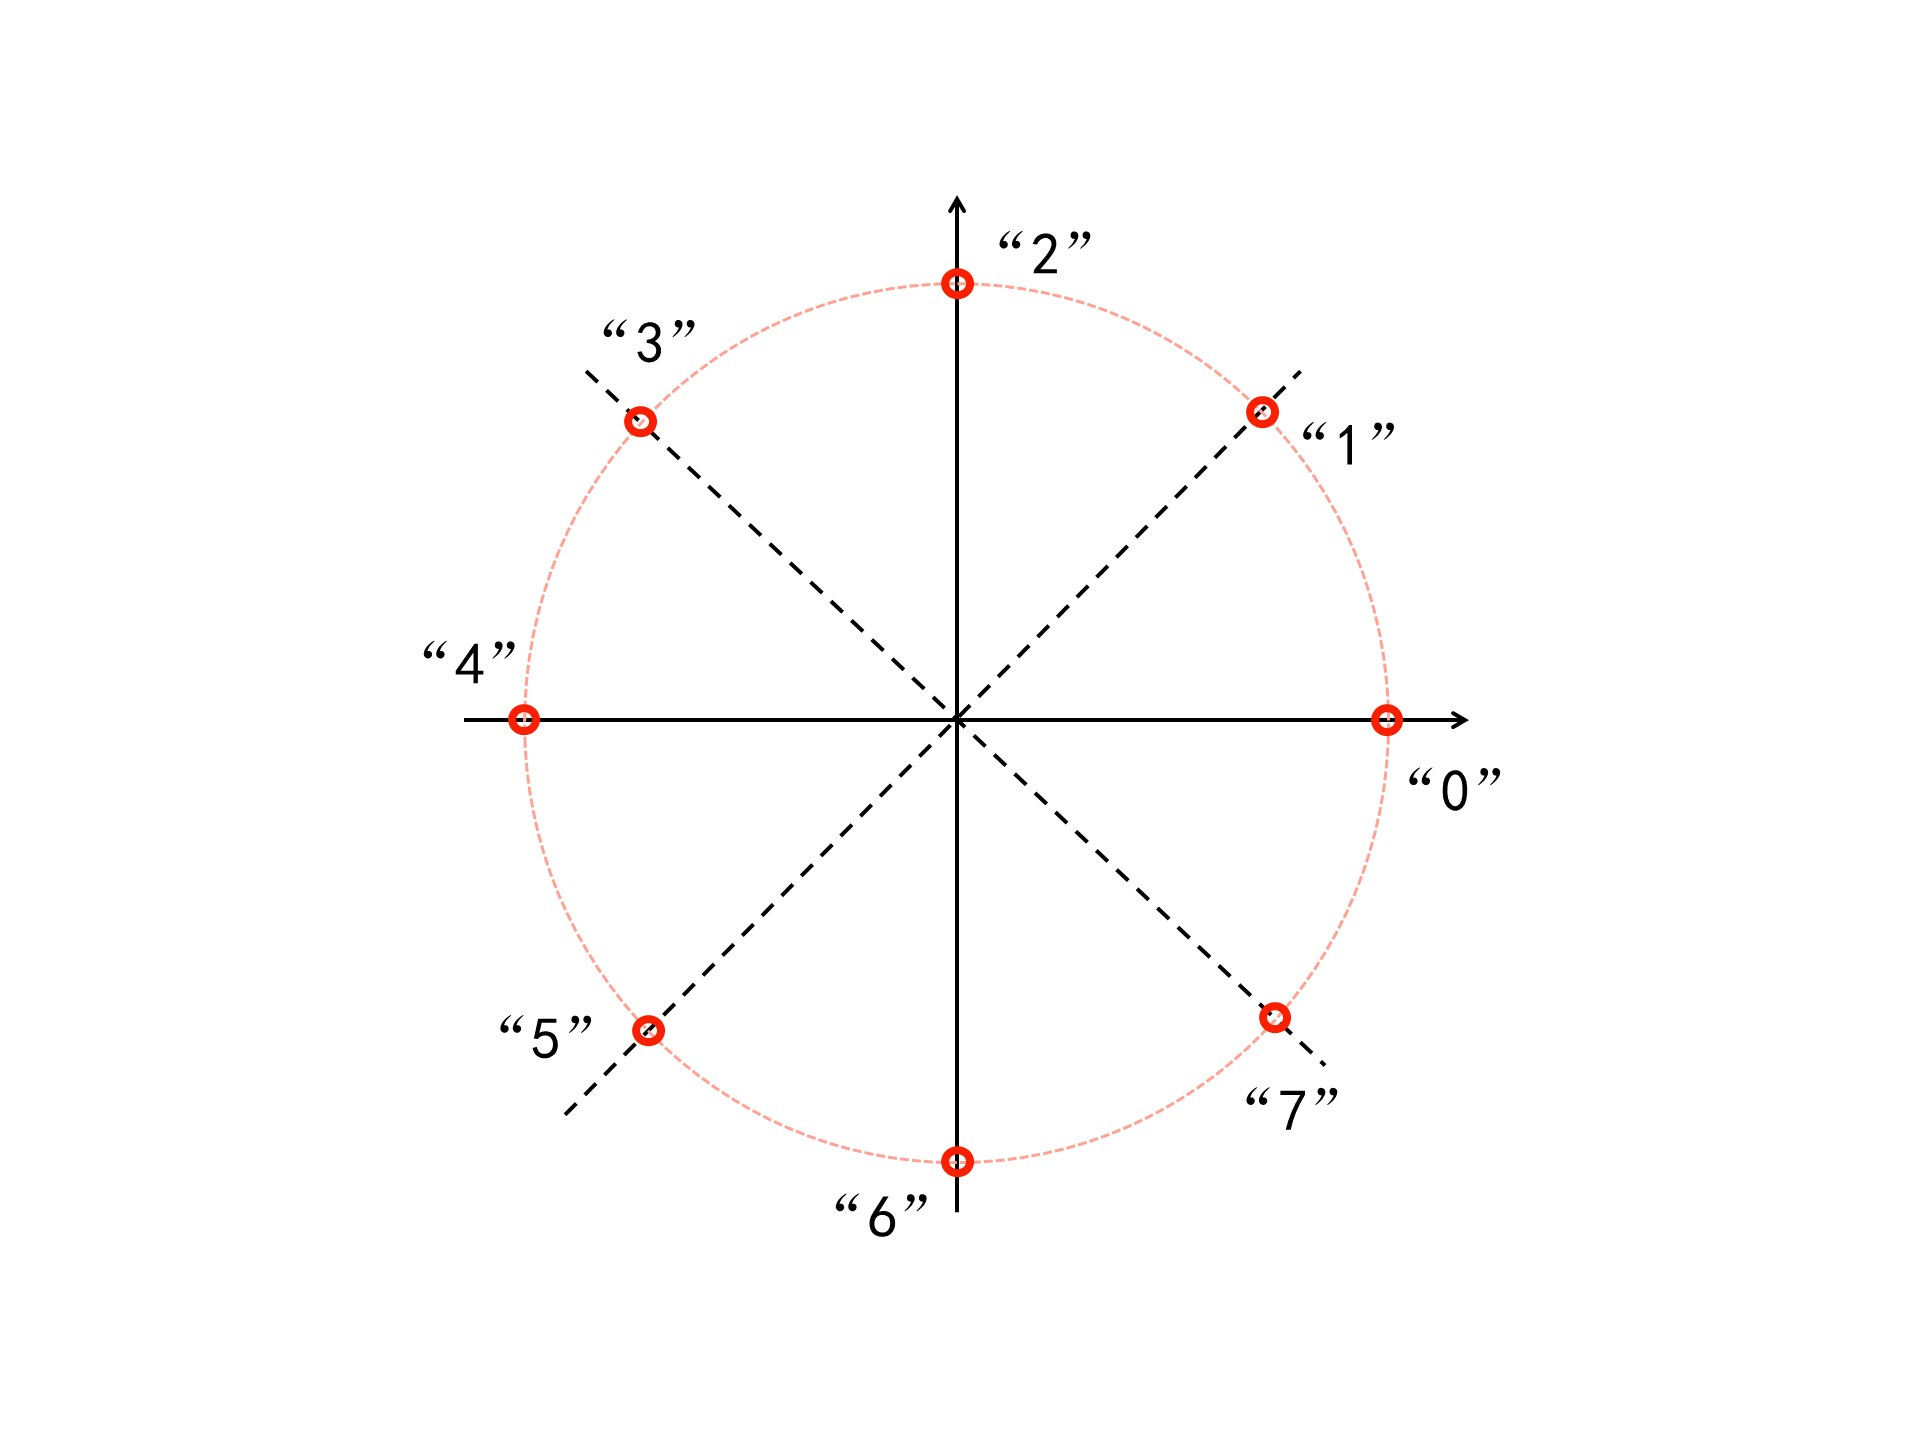
\includegraphics[width=6cm]{pic/8qpsk.jpg}
%\caption{8QPSK}
%\label{8qpsk}
%\end{figure}

\subsection{Analog input -- Vectors}

\section{C-NOT gate}
With the help of a C-NOT gate, the 2 bits of information modulated in one qubit can be transfered to two qubits and therefore can be all extracted.

\section{Phase kick back}
With the help of a C-NOT gate, the 2 bits of information modulated in one qubit can be transfered to two qubits and therefore can be all extracted.

\section{The output of Deutsch's algorithm}
With the help of a C-NOT gate, the 2 bits of information modulated in one qubit can be transfered to two qubits and therefore can be all extracted.

\subsection{Circuit diagram}
\begin{figure}[ht]
\begin{quantikz} %[wire types={q,c}]
    \lstick{\ket{0}} & \qw & \gate{H}  \slice{BS1} & \gate{f} & \ctrl{1} \slice{f()}  & \gate{H} & \meter{} &\cw \rstick{F(0)+F(1)} \\
    \lstick{\ket{0}} & \gate{X}  & \gate{H} & \qw & \gate{X} &\qw \rstick{\ket{BS2}}
\end{quantikz}
\begin{quantikz} %[wire types={q,c}]
    \lstick{\ket{0}} & \qw & \gate{H}  \slice{BS1} &\gate[2]{U_f} \slice{f()}  & \gate{H} & \meter{} &\cw \rstick{F(0)+F(1)} \\
    \lstick{\ket{0}} & \gate{X}  & \gate{H} & &\qw \rstick{\ket{BS2}}
\end{quantikz}
\caption{Deutsch's algorithm circuit}
\label{Deutsch1}
\end{figure}

\subsection{Performance}
Processing: one function $f(x)$ evaluation.
Storage: one qubit for the processing. But the measurement requires two qubit.

\section{Superdense coding}
Superdense coding is also called dense coding. With the consideration of two qubits as one wave, modulation of one qubit is modulating the shared $\theta$ of the entanged wave. The modulation appears to be upon one qubit. But the information is actually coded into two qubits.

The operation first creates entanglement $|BES1>$.

\begin{table}[]
\caption{Modulate one qubit to encode 2 bits}
\label{DenseCodingTable}
\begin{tabular}{lll}
Digital input & Modulating operation & gate                 \\
00 & None   & None \\
01 & $90 degree$& Z gate \\
10 & Mirror switch $|0>$ and $|1> $ &X gate \\
11 & Mirror switch $|0>$ and $|1>$ and $90 degree$ &X gate
\end{tabular}
\end{table}

\subsection{Circuit diagram}
\begin{figure}[ht]
\begin{quantikz}%[slice all, slice style={shorten <=8mm}, slice label style = {yshift=-38mm} ]
    & & &\lstick{Alice' 2nd bit}  & \cwbend{2} \\
    & & \lstick{1st bit}  & \cwbend{1} \\
    \lstick{\ket{0}} & \gate{H} &\ctrl{1} & \gate{Z} & \gate{X} &\ctrl{1} & \gate{H} & \meter{} &\cw \rstick{Bob's 1st bit} \\
    \lstick{\ket{0}} & \qw      & \targ{} \slice[style={shorten <=12mm}, label style={yshift=-38mm}]{BS1} & \qw \slice[style={shorten <=12mm}, label style={yshift=-38mm}]{BS2} & \qw \slice[style={shorten <=12mm}, label style={yshift=-38mm}]{BS3} & \targ{} & \qw & \meter{} & \cw \rstick{Bob's 2nd bit}
\end{quantikz}
\caption{Superdense coding circuit}
\label{DenseCoding}
\end{figure}

\subsection{Entanglement and measurement}

\section{Teleportation}
Similar to dense coding, quantum teleportation is to modulate an analog signal to one qubit of a $|BS1>$ two-qubit wave. The analog signal comes in the form of a qubit, which we call it the signal qubit. And the wave may be written as $a |0> + b|1>$.
\begin{equation}\label{}
\begin{array}{rl}
    & (a |0> + b|1>) \frac 1 {\sqrt 2}(|0>|0>+|1>|1>) \\
    = & \frac 1 {\sqrt 2}| (|0>|0>+|1>|1>) (a |0> + b|1>) \\
    +& \frac 1 {\sqrt 2}| (|0>|0>-|1>|1>) (a |0> - b|1>) \\
    +& \frac 1 {\sqrt 2}| (|0>|1>+|1>|0>) (a |0> + b|1>) \\
    +& \frac 1 {\sqrt 2}| (|0>|1>-|1>|0>) (a |0> - b|1>)
\end{array}
\end{equation}

\begin{table}[]
\caption{Modulate one qubit to encode 2 bits}
\label{TeleportationTable}
\begin{tabular}{ll}
Alice's output $d_1 d_0$ & Bob's qubit  \\
00 & $a|0>+b|1>$ \\
01 & $a|1>+b|0>$ \\
10 & $a|0>-b|1>$  \\
11 & $a|1>-b|0>$ 
\end{tabular}
\end{table}

Alice has a qbit with information S and shares a pair of qbits with Bob. The pair is one of the 4 known eigenwaves and has information 2. The total input information is therefore S+2. At the output, Alice measures the first 2 qbits against the same 4 eigenwaves and tells Bob the result, which has information 2. If no information is lost, the information in the 3 qbit should be S.

\subsection{Circuit diagram}
\begin{figure}[ht]
\begin{quantikz}%[slice all, slice style={shorten <=8mm}, slice label style = {yshift=-38mm} ]
    & & \lstick{Alice' wave a\ket{0}+b\ket{1}}  & \ctrl{1} & \gate{H} & \meter{} &\cw \rstick{Alice' 1st bit} \\
    \lstick{\ket{0}} & \gate{H} &\ctrl{1} & \targ{} & \qw& \meter{} &\cw \rstick{Alice' 2nd bit} \\
    \lstick{\ket{0}} & \qw      & \targ{} \slice[style={shorten <=2mm}, label style={yshift=-38mm}]{BS1} & \qw \slice[style={shorten <=2mm}, label style={yshift=-38mm}]{BS2} & \qw \slice[style={shorten <=2mm}, label style={yshift=-38mm}]{BS3} & \qw \rstick{Bob's wave}
\end{quantikz}
\caption{Teleportation circuit}
\label{Teleportation}
\end{figure}

\section{Quantum secure direct communication (QSDC)}
QSDC is an adaptation of quantum teleportation to key distribution. The key transmission rate is 1 bit per qubit duty cycle and is a much improvement over the BB84 protocol.

\chapter{n-qubit operations}

\section{Grover's algorithm}
Like the Deutsch's algorithm, the Grover's algorithm also assumes a blackbox function $f(x)$ whose variable $x$ is a $n$-bit binary variable. Its result is a single-bit value and is always 1 except for an unknown $x=x_w$ at which $f(x_w)=-1$. The goal of the algorithm is to find $x_w$. This is the simplified version of many search problems. Lov Grover proposed in 1996 that quantum computer can solve it faster than conventional computers.

Let's note $x_w$ as $w_{n-1}...w_i...w_1 w_0$ in binary where $w_i = 0 or 1$, and $\Vec{w} = (0, 0, ..., 1 at i=w, ..., 0)^T$ as a $2^n-1$ dimensional vector. Using classical computers, we'd feed each of the $2^n -1$ possible numbers of $x_w$ at a time to $f$ to test whether the result equals $-1$. The worst case is that we have to do $2^n-1$ evaluations of $f(x)$ to find out $x_w$. We of course wish to explore all the possible $x_w$ at the same time. We naturally choose $\vec{S} = \frac 1 {\sqrt{2^n}} (1, 1, ...1)^T$, which is the sum of all the bases of the qubits, to feed the oracle function $f$.

We know, $\vec{S} = \vec{S} - \frac 1 {\sqrt{2^n}} \vec{w}) + \frac 1  {\sqrt{2^n}} \vec{w}$. Apparently, $\vec{S_1}  = \vec{S} - \frac 1 {\sqrt{2^n}} \vec{w}$ is a vector orthogonal to $\vec{w}$, and applying the $F$ gate to it does not change its phase. Therefore, $F(\vec{S}) = F(\vec{S_1}) + F(\frac 1  {\sqrt{2^n}} \vec{w})  = \vec{S_1} - \frac 1 {\sqrt{2^n}} \vec{w}$. We see that 
\begin{itemize}
    \item applying the $F$ gate turns vector $\vec{S}$ toward $-\vec{w}$
    \item applying the $F$ gate to $\vec{S_1}$ makes no change.
\end{itemize}
Therefore, can we apply $F$ gate $2^n$ times and turn $\vec{S}$ completely to $-\vec{w}$? But applying $F$ gate once more will change the phase of the $\vec{w}$ vector back. We need to change the sign of vector $\vec{w}$ first while preserving its angle with $\vec{S}$ before applying $F$ gate again. This can be accomplished by apply gate $U_S = 2 \vec{S}X\vec{S} -I$.

\begin{figure}[ht]
\begin{tikzpicture}
\coordinate (S) at (30:3);
    \draw[red, fill] (S) circle(0.05cm)  node[right] {$\vec{S}$};
    \draw[->, dashed] (0,0) -- (S);
    \draw[->] (0,0) -- (3, 0) node[below] {$\vec{w_v}$};
    \draw[->] (0,0) -- (0,3) node[right] {$\vec{w}$};
    %\draw[dotted, red] (0,0) circle(3cm);
\end{tikzpicture}
\caption{Applying F gate}
\label{grover}
\end{figure}

\subsection{Complexity}

\section{Phase estimation}
\subsection{Complexity}

\section{Simon's algorithm}
The Simon's algorithm assumes a blackbox oracle function $f(x)$ whose variable $x$ is a $n$-bit binary variable. Its results are $m$-bit values that are periodic, but the period $t$ is unknown -- $f(x+t)=(fx)$ for all $x$. How do we find the period $t$? Of course, we are tempted to play the trick again of feeding $\vec{S} = \frac 1 {\sqrt{2^n}} (1, 1, ...1)^T$ to the oracle function $f$. We have
$f(\vec{S}) = \frac 1  {\sqrt{2^n}} \sum_x f(x)$.

\subsection{Circuit diagram}
\begin{figure}[ht]
\begin{quantikz}%[slice all, slice style={shorten <=8mm}, slice label style = {yshift=-38mm} ]
    & & &\lstick{Alice' 2nd bit}  & \cwbend{2} \\
    & & \lstick{1st bit}  & \cwbend{1} \\
    \lstick{\ket{0}} & \gate{H} &\ctrl{1} & \gate{Z} & \gate{X} &\ctrl{1} & \gate{H} & \meter{} &\cw \rstick{Bob's 1st bit} \\
    \lstick{\ket{0}} & \qw      & \targ{} \slice[style={shorten <=12mm}, label style={yshift=-38mm}]{BS1} & \qw \slice[style={shorten <=12mm}, label style={yshift=-38mm}]{BS2} & \qw \slice[style={shorten <=12mm}, label style={yshift=-38mm}]{BS3} & \targ{} & \qw & \meter{} & \cw \rstick{Bob's 2nd bit}
\end{quantikz}
\caption{Simon's algorithm}
\label{DenseCoding}
\end{figure}

\subsection{Complexity}
Using conventional computer, finding the period takes $2^{n/2}$ operations.

\section{Shor's algorithm}

\subsection{Complexity}

\section{Boson sampling algorithms}

\subsection{Complexity}

\chapter{Noise, and error correction}
\section{Channel capacity}
According to Shannon theorem, under noise, the channel capacity is $C = 2B (1+SNR)$.


\chapter{Appendix: Qubit devices}\label{A-qubit}

\section{Free space optical qubits}
Free space communication is mostly used for satellites to communicate with each other. There is no substance in space to degrade the power of the light wave. The receiver may as receive less power if the light beam diverge in a large angle. Laser lights are typically used. Free space communication can also be used for ship-ship communication if the distance is not too far resulting in high power loss.

Lights are propagating electromagnetic waves and obviously are best suited for communications. The vibration direction of the electric field of an electromagnet wave is its polarization. A free space optical qubit uses one optical wave of horizontal polarization to represent the binary number 0 and is thus label $|0>$. It uses the one of vertical polarization to represent 1 and is labeled $|1>$. The two waves have the same frequency and amplitude. They are orthogonal to each other of course. A wave of polarization angle $\theta_p$ can be considered the superposition of the two base waves: the $|0>$ wave contributes $cos\theta_p$ amount in amplitude while the $|1>$ wave contributes $sin\theta$.

Polarization modulation is also used in optical fiber communication. For example, dual polarization quadrature phase shift keying (DP-QPSK) modulation is a widely used.

\section{Superconductor qubits}
A superconductor transmon qubit is similar to the string of a guitar and uses the first two standing waves, which resonate at the first and second harmonic frequencies respectively, to represent the integers of "0" and "1". Such a qubit is constructed by two superconductors separated by a layer of insulator. The insulator is thin enough for electrons to move ("tunnel") back and forth from one superconductor to another without loss of energy. But traveling through the insulator leads to delays (phase delays) of the electrons. The back-and-forth movement (vibration) of the electrons between the two superconductors resonate as standing waves at periods fractions of the delay. typically, the first fundamental frequency and the first harmonic are used to represent "0" and "1".
\begin{figure}[ht]
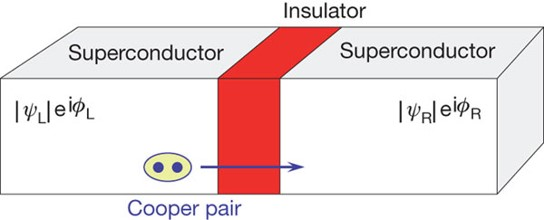
\includegraphics[width=6cm]{pic/supercQubit.jpg}
\caption{Superconductor qubit}
\label{Superconductor}
\end{figure}

\begin{figure}[ht]
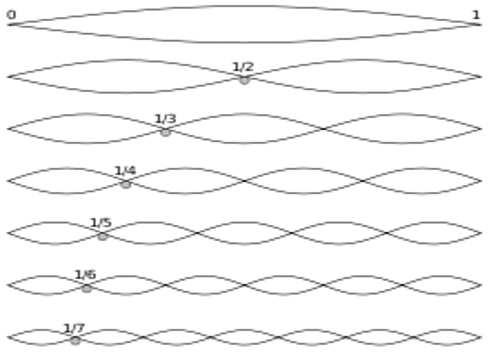
\includegraphics[width=6cm]{pic/overtones.png}
\caption{The vibration of a string is a superposition of standing waves with wavelengths fractions of the string length.}
\label{Overtones}
\end{figure}

\chapter{Appendix: Quantum gates}

\subsection{C-NOT gate}
\subsection{Phase kick back}

\subsection{Generator}
How a qubit is put in the wave of "0" or "1" depends on the specific implementation. A quantum circuit diagram is usually drawn with a qubit starts in the "0" or occasionally in the "1" wave.

\subsection{Hadamard gate}
To modulate a qubit in the 10 or 11 wave, a $\theta_pm = 45$ degree phase shifter in the constellation diagram is needed. In the Bloch sphere, a $\theta_q =90, \phi=0$ phase shift is needed. Such a phase shifter is called a Hadamard gate. In the ket notation, $|11> = 1 over [\sqrt 2] (|0> + |1>)$ and $|10> = 1 over [\sqrt 2] (|0> - |1>)$. So, as a vector transformation, the Hadamard gate is a transformation matrix:
\begin{equation}
    \frac 1 {\sqrt 2}
    \begin{pmatrix}
1 & 1 \\
1 & -1
\end{pmatrix}
\end{equation}

\chapter{Bibliography}
\bibliographystyle{unsrt}
   \bibliography{qcc}

\backmatter
\addcontentsline{toc}{chapter}{Index}
\printindex
\end{document}